\documentclass[10pt]{ruthesis}
\special{papersize=8.5in,11in}
\usepackage{natbib}
%\usepackage{aastex_hack,deluxetable} 
\usepackage{graphicx,subfigure,hyperref}
%\usepackage{rotating}
\usepackage{lscape,longtable,float}
\setlength{\unitlength}{1.0cm}
% Load packages; ambssymb is for extra fonts, such as blackboard
\usepackage{latexsym}
\usepackage{amsmath}
\usepackage{amssymb}
\usepackage{amsbsy}
\usepackage{braket}
\usepackage[bottom]{footmisc}
% Define Italic Sans Serif font (for tensors)
\DeclareMathAlphabet{\mathsfsl}{OT1}{cmss}{m}{sl}

%\draft

\begin{document}
\phd 
\title{PhD Thesis Draft}
\author{Bismayan Chakrabarti}
\program{Physics and Astronomy}
\director{Prof. Kristjan Haule}
\approvals{5}
\submissionyear{2017}
\submissionmonth{January} 
%\setcounter{tocdepth}{1}
\abstract{ The study of strongly correlated materials is currently perhaps one of the most active areas of research in condensed matter physics. Strongly correlated materials contain localized electronic states which are often hybridized with more itinerant electrons. This interplay between localized and delocalized degrees of freedom means that these compounds have highly complex phase diagrams which makes these compounds very challenging to understand from a theoretical standpoint. Computer simulations have proved to be an invaluable tool in this regard with state of the art ab-initio simulation techniques harnessing the ever-increasing power of modern computers to produce highly accurate descriptions of a variety of strongly correlated materials. One of the most powerful simulation techniques currently in existence is Dynamical Mean Field Theory (DMFT). This thesis describes this powerful simulation technique and its applications to various material systems, as well as addressing some theoretical questions concerning particular implementations of DMFT.


This thesis is divided into two parts. In part 1, we describe the theory behind DMFT and it's amalgamation with Density Functional Theory (DFT+DMFT). In chapters 2 and 3, we provide the basic theory theory behind DFT and DMFT respectively. In chapter 4, we describe how these two methods are merged to give us the computational framework that is used in this thesis, namely DFT+DMFT. Finally, we round off part 1 of the thesis in chapter 5, which provides a description of the Continuous Time Quantum Monte Carlo (CTQMC) impurity solver, which is at the heart of the DFT+DMFT algorithm and is used extensively throughout this thesis. 


In part two of the thesis, we apply the DFT+DMFT framework to address some important problems in condensed matter physics. In chapter 6, we study the Magnetic Spectral function of strongly correlated f-shell materials to understand two important problems in condensed matter physics, namely the volume collapse transition in Cerium and the valence fluctuating state ground state of $\delta$-Pu. In chapter 7, we study the contribution of lattice parameters and electronic entropy to study the decades-old problem of understanding the spin state transition observed in $\mathbf{LaCoO_3}$, where we show how lattice expansion, octahedral rotations and electronic entropy are all essential in stabilizing the high-spin state at high temperature. In chapter 8, we switch to studying a more theoretical problem by looking at the problems with using the highly popular constrained Random Phase Approximation (cRPA) method to estimate the screening of local inter-electronic repulsion in strongly correlated systems. We show that cRPA systematically underestimates screening in such systems which makes it an unsuitable method for estimating the repulsion parameter (U) used in impurity solvers. We then develop an alternate method to estimate the screening using the full local polarization which overcomes many of these limitations. Chapter 9 contains all  the conclusions obtained in this thesis, followed by references and appendices. 

 
}

\beforepreface
\acknowledgements{I would like to start by thanking Prof. Kristjan Haule for all the help provided by him over the course of my Ph.D. None of this work would have been possible without his constant support, intellectual freedom, guidance as well the computational resources provided by him. 

I would also like to thank Prof. Gabriel Kotliar, for all the help he has so freely provided as well as his valuable insight which I have gained a lot from, especially during my study of magnetic spectrum of f-shell materials.

I have gained most of my expertise in physics from the courses taught here at Rutgers by the highly knowledgeable faculty in the physics department. I would like to the thank all the professors I have taken courses with, as well the entire faculty of the condensed matter department who have always inspired me with their great dedication to constantly pushing the limits of human knowledge.

Over the course of my dissertation, I have had the opportunity to work with a number of highly talented post-doctoral scholars and doctoral students whom I have collaborated closely with. Dr. Maria Pezzoli was a great help during my initial research on magnetic properties of materials. Dr. Turan Birol has been a constant source of help and support over the last three years of my research and I have gained a lot from his knowledge of physics and life in general. Dr. Chuck Hou Yee has also been a trusted friend and colleague who has always been available whenever I had a question about physics, science or computation in general. Qiang Han and I had a great experience working on the project estimating screening in correlated systems and I wish him the best in all his future endeavors. 

In addition to this,the Rutgers has also provided me with a valuable set of friends who have made my experience as a graduate student a lot more enjoyable. To Aniket, Juho,Patrick, Conan, Upamanyu, Dinesh, Kartik, Rahul, Hitesh, Kinnari, Shree, Samruddhi and all the other friends I have been fortunate enough to make at Rutgers, I would like to thank all of you for all the immensely enjoyable experiences which have made my time at Rutgers some of the best years of my life.

Finally, I would like to thank my parents, my sister and my entire extended family for always being there for me whenever I have needed them. Your love and support inspires me to always strive for perfection in whatever I do and I am truly lucky to have been been born into a family which has such kind and loving individuals.  
}
\dedication{
\begin{center}
{To my family and friends} \\
\end{center}
}
\figurespage
\tablespage
\afterpreface

% aliases begin
\newcommand{\Ps}{\Psi}
\newcommand{\ps}{\psi}
\newcommand{\da}{\dagger}
\newcommand{\la}{\langle}
\newcommand{\ra}{\rangle}
\newcommand{\rmb}{\mathbf{r}}
\newcommand{\kmb}{\mathbf{k}}
\newcommand{\dens}{n(\rmb)}
\newcommand{\cdag}{c^{\dagger}}
\newcommand{\upa}{\uparrow}
\newcommand{\dow}{\downarrow}
\newcommand{\sig}{\sigma}
\newcommand{\ib}{\int_{0}^{\beta}}
\newcommand{\eps}{\epsilon}
\newcommand{\vR}{{\mathbf{R}}}
\newcommand{\vr}{{\mathbf{r}}}
\newcommand{\hr}{{\hat{\textbf{r}}}}
\newcommand{\vk}{{\mathbf{k}}}
\newcommand{\vK}{{\mathbf{K}}}
\newcommand{\vq}{{\mathbf{q}}}
\newcommand{\vQ}{{\mathbf{Q}}}
\newcommand{\vPhi}{{\mathbf{\Phi}}}
\newcommand{\vS}{{\mathbf{S}}}
\newcommand{\cG}{{\cal G}}
\newcommand{\cF}{{\cal F}}
\newcommand{\cT}{{\cal T}}
\newcommand{\cH}{{\cal H}}
\newcommand{\cJ}{{\cal J}}
\newcommand{\cD}{{\cal D}}
\newcommand{\cL}{{\cal L}}
\newcommand{\Tr}{\mathrm{Tr}}
\renewcommand{\a}{\alpha}
\renewcommand{\b}{\beta}
\newcommand{\g}{\gamma}
\renewcommand{\d}{\delta}
\newcommand{\npsi}{\underline{\psi}}
\renewcommand{\Im}{\textrm{Im}}
\renewcommand{\Re}{\textrm{Re}}
\newcommand{\cA}{{\cal A}}

% aliases end


\pagebreak

\chapter{Introduction}

Condensed Matter Physics involves the scientific study of the macroscopic properties of materials. In a rich history spanning a century since the birth of quantum mechanics, Condensed Matter physics has grown into one of the most active fields of physics and has had a direct role in enabling the technological revolution that the human species is currently living through. In most fields of physics, the fundamental concept which underlies most research is that of ``Reductionism", which is the belief that every phenomenon can be explained by understanding the fundamental properties of its most elementary constituents. However, the basic philosophy of  condensed matter physics is perhaps best summarized by the oft-quoted phrase coined by P.W Anderson- "More is different". It captures the idea that a macroscopic collection of constituent elements exhibits properties which are hard to predict based on merely the microscopic equations governing the individual constituents. This idea, which is known ``emergence", is what condensed matter physicists strive to understand in the realm of the quantum properties of materials. Examples of emergent properties (see Fig 1.1) include water molecules forming complex waves in water bodies and intricately shaped snow flakes in winter, swarms of living organisms exhibiting behaviors much more complicated than individual members, or perhaps most stunningly, how a collection of lifeless chemical elements can combine to form something as complex as a human being. In condensed matter, the study of emergent properties in material systems has given us a keen understanding of why a material might behave as a metal,insulator, semiconductor,magnet, superconductor or a variety of other complex phases known to us, even though it might be composed of very similar elements. The ability to understand and thereby control these material properties have resulted in condensed matter physics having a great impact in engineering and technology, making it a field of physics which has a pronounced real-world impact in society.
\linebreak
\begin{figure}[H]
\includegraphics[width=\columnwidth]{Emergence.jpg}
\caption{Examples of Emergent behavior in nature: (from left) 1) swarms of birds displaying complex behavior. 2) Snowflakes of complex different shapes formed by the same fundamental solid phase of water \protect \footnotemark  }

\end{figure}
\footnotetext{Sources-1) fuelspace.org 2) Wikipedia}

Within condensed matter, one of the most active and fascinating fields is the study of strongly correlated systems. In most materials (like those where the constituent elements all have open s and p shells), the somewhat naive yet powerful approximation that the electrons in the material act as independent particles moving in an effective medium, known as the independent electron approximation works surprisingly well. This effect, which is explained by the Landau Fermi Liquid Theory, occurs due to these extremely mobile itinerant electrons forming "quasiparticles", which result in the inter-electronic coulomb repulsion being screened highly effectively. This success of the Landau Fermi liquid theory and other theoretical approximation schemes has meant that we have quite a good understanding of the properties of these ``weakly correlated systems" (though some particular systems still remain challenging).

However this approximation usually breaks down in materials with incomplete d and f shells, because the electrons in these shells are localized to a much greater extent around their parent atoms (see Fig 1.2). These electrons cannot effectively screen each other, unlike the much more itinerant s and p electrons and therefore retain some of their atomic properties. In addition, there is often strong mixing (hybridization) between them and the outer s and p electrons, leading to a large interplay between itinerant and localized degrees of freedom. Such materials, commonly known as \textit{strongly correlated systems}, often have highly complex phase diagrams with many different phases across which transitions can be tuned by tweaking some external \textit{knob} such as temperature or pressure. This makes these systems particularly useful from a material science/engineering standpoint.

\begin{figure}[H]
\includegraphics[width=\columnwidth]{Knetko-Smith.jpg}
\caption{The Kmetko-Smith diagram showing the trends in increasing electronic correlation/localization across different shells of the periodic table. The elements at the bottom left corner display the least amount of correlations and form conventional superconductors at low temperatures. At the other extreme elements in top right corner show extremely high localization and typically form local moments which give rise to magnetism \protect \footnotemark}

\end{figure}
\footnotetext{Source- Introduction to Many-Body Physics. Piers Coleman (Cambridge University Press)}

Finding a coherent theoretical framework which can capture the essential properties of such complex materials has proved to be immensely challenging and continues to be an area of active research. Computational simulations have played an important role in this effort and have enabled us to study and predict properties of real materials instead of restricting ourselves to model Hamiltonians. These developments have been made possible by large improvements in both the hardware capabilities of modern computers as well as the development of new faster and more powerful simulation algorithms. In the field of weakly correlated materials, Density Functional Theory (DFT) has led to a revolution in material simulation, and has given us the power to compute properties using relatively modest computational resources, which has led to an explosion in research in computational materials physics as well as quantum chemistry. However DFT, while being extremely powerful, is often completely inadequate when applied to strongly correlated systems, as the drastic approximations it employs  contain only rudimentary treatments of the electronic correlations which are essential to understanding the physics of these compounds (for more details refer to chapters 2 and 3).

Dynamical Mean Field Theory (DMFT) is one of the most promising theories which aims to address some of these shortcomings. DMFT provides us a way to simulate strongly correlated systems using controlled approximations which reduce the computational complexity while retaining most of the essential physics of the system, including the interplay between itinerant and localized degrees of freedom. This method, which initially became popular as a method to solve model Hamiltonians such as the Hubbard Model, has proved to be a valuable tool to capture the properties of d and f shell systems. This has especially been true in the last decade after the successful merger of DMFT with DFT to yield a framework which is capable of dealing with both the weakly correlated electrons (which DFT is well suited to) as well as the localized d and f orbital electrons, where DMFT shines. This approach, known as DFT+DMFT has proved to be one of the most successful methods in reproducing experimentally verifiable properties of correlated systems and is one of the methods driving the advancement in human understanding in the field of correlated materials .

As result of these and other highly advanced computational techniques available, computational condensed matter today is one of the most exiting fields of physics to be part of. The current algorithms allow us , for perhaps the first time in history, to perform "computational experiments", where we can simulate materials reliably and quickly given sufficient computational resources. It is hoped that soon this would give us the power to perform computational material design, which is perhaps one of the ultimate aims of condensed matter physics. We could soon be at a stage where we can solve the inverse problem of having been given a certain set of desired properties, of being able to predict which exact chemical system would satisfy those requirements from first principles without necessarily having to resort to actual experimentation. Since strongly correlated materials display some of the most interesting properties known in nature, it is to be expected that methods such as DFT+DMFT will be at the cutting edge of such efforts. 

In this thesis, we shall study some of the fundamental theoretical aspects of the DFT+DMFT method as well as its applications to real material systems. The thesis is arranged in the following manner: In Part 1 , we shall aim to present a description of the theory behind DFT+DMFT. In chapter 2 we shall give a brief introduction to Density functional Theory (DFT) and the equations which govern the method. In chapters 3 and 4, we shall explain the DMFT method, provide details of the exact approximations and explain how the merger of DFT+DMFT is carried out in practice. In Chapter 5 we shall provide more technical details of the Computational algorithm which lies at the heart of our implementation of DFT+DMFT, the Continuous Time Quantum Monte Carlo (CTQMC) impurity solver. Having laid out the major theoretical building blocks of our framework, in Part 2 we shall move on to particular problems which have been investigated in the course of this doctoral study. Chapter 6 details the investigation of the magnetic spectral function of f-shell compounds such as $\alpha$ Cerium, $\gamma$ Cerium and $\delta$ plutonium. Chapter 7 describes a study of the the importance of structural parameters and electronic entropy in the spin state transition in $LaCoO_3$ using DFT+ DMFT. Chapter 8 contains the investigation of the inadequacy of the Constrained Random Phase Approximation(cRPA), one of the most popular methods to estimate screening in strongly correlated systems. Chapter 9 contains the conclusion and is followed by the Bibliography and Appendices.


\pagebreak
\chapter{Density Functional Theory}

Density Functional Theory(DFT) is one of the most successful theories in the world of modern physics. Its immense popularity can be gauged from the fact that the seminal papers  by Hohenberg and Kohn \cite{Hohenberg_Kohn}, and Kohn and Sham \cite{Kohn_Sham} are the two most heavily cited papers in modern times. Density functional theory allows for ab-initio (with no arbitrary tunable free parameters) calculations of the zero-temperature ground state material properties of the vast majority of weakly correlated compounds. With the growth of modern algorithms in this field, one can now employ off-the-shelf packages to obtain highly accurate results for a large variety of experimental observables while spending very little computational resources. In this section, we shall concentrate on giving a brief introduction to the principles of DFT, while also mentioning some of the limitations that have led to the search for more advanced methods.

As a starting point for the discussion, we begin with the "Theory of everything" for condensed matter systems, describing a non-relativistic lattice system of nucleii and the accompanying electrons:
\begin{equation}\label{DFT_1}
H=-\dfrac{\hbar^2}{2m_e}\sum_i\nabla_i^2  -\dfrac{\hbar^2}{2M_e}\sum_I\nabla_I^2 +\dfrac{1}{2}\sum_{i\neq j} \dfrac{e^2}{|\rmb_i -\rmb_j|}-\dfrac{1}{2}\sum_{i, I} \dfrac{e^2Z_I}{|\rmb_i -\mathbf{R}_I|} + \dfrac{1}{2}\sum_{I\neq J} \dfrac{e^2Z_I Z_J}{|\mathbf{R}_I -\mathbf{R}_J|} 
\end{equation}
In this equation, the first two terms describe the kinetic energy of the nucleii and the electrons respectively while the next three terms describe the inter-nuclear, nuclei-electron and electron-electron Coulomb interactions. Note that this equation neglects relativistic corrections such as spin orbit coupling which can become important in some systems (and which most advanced DFT packages are able to treat to some degree). We first simplify this equation by adopting the so-called Born-Oppenheimer approximation, whereby the nucleii are assumed to be fixed. This is exceptionally accurate due to the relatively much higher mass of the nucleii compared to the electrons. This approximation dispenses with the nuclear kinetic energy term and leaves us with a Hamiltonian for the electrons moving in an effective field created by the lattice of nucleii. This resulting Hamiltonian is-
\begin{equation}\label{DFT_2}
H=-\dfrac{\hbar^2}{2m_e}\sum_i\nabla_i^2 + \dfrac{1}{2}\sum_{i\neq j} \dfrac{e^2}{|\rmb_i -\rmb_j|} +\sum_i V_{ext}(\rmb_i) +E_{ion}
\end{equation}

Where $E_{ion}$ is the constant inter-nuclear Coulomb term and $V_{ext}$ is the nucleii-electron repulsion given by-

\begin{equation}
 V_{ext}(\rmb)= \sum_{I} \dfrac{e^2 Z_I}{|\rmb-\mathbf{R}_I|}
 \end{equation} 

However, even this simplified many-electron Schrodinger equation is essentially impossible to solve for more than O(10) electrons. The major breakthrough, first proposed by Hohenberg and Kohn \cite{Hohenberg_Kohn} was to show that, at least for the calculation of ground state properties, it is sufficient to work with the charge density rather than the wave function itself. Or in other words, the ground state wavefunction and other observables are uniquely determined  by the charge density-
\begin{equation}
n(\rmb)= \la \Ps|\ps^\da (\rmb) \ps(\rmb) | \Ps\ra 
\end{equation}
Note that this leads to enormous decrease in computational complexity, $n(r)$ is a 3 dimensional scalar instead of the original 3N dimensional vector $\Ps$.  The result is proved most easily by contradiction. Let us assume that two different external potentials $V_{ext} (r)$ and $V'_{ext} (r)$ produce the same charge density $n(r)$
when plugged into Eq. \ref{DFT_2}. If we denote these two Hamiltonians $H$ and $H'$ ,their ground state wavefunctions $\Ps$ and $\Ps'$ and the corresponding ground state energies $E$ and $E'$, then without loss of generality we can say
\begin{equation}
E'=\la \Ps' | H' |\Ps' \ra < \la \Ps | H' |\Ps \ra = \la \Ps | H' + V'_{ext} (\rmb) -V_{ext} (\rmb)   |\Ps \ra
\end{equation}
where the inequality comes from the fact that $\Ps$ is not the ground state of $H'$. From this, we get
\begin{equation}
E < E' + \int d\rmb \left( V'_{ext} (\rmb) -V_{ext}(\rmb) \right) n(\rmb)
\end{equation}
Since both external potentials give the same charge density, exchanging the primed and unprimed dummy indices, we get
\begin{equation}
E' < E + \int d\rmb \left( V_{ext} (\rmb) -V'_{ext} \right) n(\rmb)
\end{equation}
Adding these two equations, we get the obvious contradiction
\begin{equation}
E+E' < E+E'
\end{equation}
 Which proves that $V_{ext}$ (and therefore $\Ps$) is uniquely determined by the charge density.

The other theorem proved by the authors in their paper proves the existence of   a universal functional of the charge density $F[n]$ for which the functional
\begin{equation}
E[n]=F[n] +\int d \rmb n(r) V_{ext}(\rmb) + E_{ion} 
\end{equation}
attains a minimum for the ground state density, and has the value corresponding to the ground state energy at this point. The proof is relatively simple and can be formulated by identifying $F[n]$ as the part of the Hamiltonian given by Eq. \ref{DFT_2} containing the electronic kinetic and Coulomb interaction terms. Knowledge of the exact formulation of this functional would reduce the solution of any chemical system (at least the ground state properties) to a minimization problem involving only one 3-dimensional quantity (the charge density). The only component of $F[n]$ for which an exact formulation can be found is the "Hartree" component. The functional is then redefined as:
\begin{equation}
 F[n]= \dfrac{e^2}{2}\int d\rmb d\rmb' \dfrac{n(\rmb) n(\rmb')}{|\rmb-\rmb'|} + I[n]
 \end{equation} 
Where $I[n]$ contains everything in $F[n]$ not including the Hartree term, including the kinetic energy and the non-Hartree potential energy contributions. Therefore the central problem of solving any chemical system is the formulation of an accurate $I[n]$.

The first successful attempt at approximating $I[n]$, without which the findings of Hohenberg and Kohn would have remained a mere theoretical exercise, was achieved by Kohn and Sham \cite{Kohn_Sham} in their seminal paper. They proposed breaking up $I[n]$ as follows:
\begin{equation}
 I[n]=T_s[n]+E_{XC}[n]
 \end{equation} 
where $T_s[n]$ is the kinetic energy of an auxiliiary non-interacting electron system and $E_{XC}[n]$ is known as the "exchange-correlation" energy of the interacting system. $E_{XC}[n]$ was approximated as:
\begin{equation}
E_{XC}[n]=\int d\rmb \dens \epsilon_{XC}(\dens)
\end{equation}
$\epsilon_{XC}(\dens)$ is the exchange correlation energy per electron of a uniform electron gas which can be computed highly accurately using Quantum Monte Carlo simulations. This approximation of using the charge density of a uniform electron gas is Local Density Approximation(LDA) and is perhaps single handedly revolutionizing computational solid state Physics. 

In practice, DFT is implemented by  assuming the following Hamiltonian for N independent electrons:

\begin{equation} \label{KS1}
H=\sum_{i}^{N} \left[ -\dfrac{\hbar^2}{2m_e}\nabla_i^2 +V_{KS}(\rmb_i)\right]
\end{equation}

 where $V_{KS}$ is the Kohn-Sham Potential which will be derived later. We then find the N lowest eigenstates and eigenenergies of this hamiltonian, which we denote by $|\psi_i\ra$
 and $|\epsilon_i\ra$ respectively. These $\psi_i$'s allow us to calculate the charge density given by:
 \begin{equation}\label{den}
 \dens=\sum_{i=1}^{N} |\psi_i|^2
 \end{equation}
  Note that this charge density is still the charge density of the auxilliary non-interacting system defined by Eq. \ref{KS1}. This formulation though allows us to calculate $T_s[n]$ for this system using the auxilliary wavefunctions $\psi_i$'s by using the standard expression
 \begin{equation}
 T_s[n]=-\dfrac{\hbar^2}{2m_e} \sum_{i=1}^{N} \int d\rmb \psi^*_i(\rmb) \nabla^2 \psi_i(\rmb)
 \end{equation}
 
 Now we have to ensure that $V_{KS}$ is chosen such that the ground state energy of the Hamiltonian defined in Eq. \ref{KS1} corresponds to the stationary value of the Hohenberg-Kohn functional. To ensure this, we vary the functional against  $\psi$:
 \begin{equation}
  \dfrac{\delta}{\delta \psi_i^*}\left( E[n] - \sum_{j=1}^{N} \epsilon_j (\psi^*_j \psi_j -1) \right)=0
  \end{equation} 
  where $\epsilon_j$ ensures normalization of the wavefunctions. The solutions to this equation correspond to Eq. \ref{KS1} as long as the Kohn-Sham potential is defined to be
 \begin{equation}\label{KS_2}
 V_{KS}(\rmb)=V_{ext}(\rmb) + \int d\rmb' \dfrac{e^2}{|\rmb -\rmb'|} n(\rmb') + \dfrac{d E_{XC}(\rmb)}{d\dens}
 \end{equation}

Therefore we have successfully transformed the solution of the original interacting system to the solution of an auxilliary non-interacting eigenvalue problem. The problem however is nonlinear due to the implicit dependence of $V_{KS}$ on $\dens$ and thereby on the eigenfunctions themselves. The solution is therefore found iteratively, where we perform the following steps till self-consistency:
\begin{enumerate}
\item start with an initial guess for the density $\dens$
\item use it to construct $V_{KS}$ using Eq. \ref{KS_2}
\item Solve the eigenvalue problem for the Hamiltonian given by Eq. \ref{KS1} to obtain $\psi_i$ and $\epsilon_i$ 
\item Construct new $\dens$ using Eq. \ref{den} and go back to step 2
\end{enumerate}

From the converged solution, we calculate the ground state energy by :
\begin{equation}
E=\sum_i \epsilon_i - \dfrac{e^2}{2}\int d\rmb d\rmb' \dfrac{n(\rmb) n(\rmb')}{|r-r'|} +E_{XC}[n] -\int d \rmb n(\rmb) V_{XC}(\rmb)
\end{equation}
It is to be noted that that apart from the ground state, the eigenvalues and eigenfunctions of the Kohn Sham Hamiltonian are meaningless, strictly speaking. However in practice they are often found to be in good agreement with experimental bandstructures and are used as such.

So we see that Density Functional Theory provides us with a valuable tool with which to perform ab-initio simulations of real materials. The success of this method is mainly based on its computational efficiency and ease of implementation, which has resulted in a number of packages being developed such as VASP \cite{Vasp}, Quantum Espresso \cite{Quantum_Espresso}, Abinit \cite{Abinit} and Wien2k \cite{wien2k} which offer off-the-shelf implementations which enable researchers to perform reliable and fast simulations even with very limited resources. However DFT fails when applied to materials with strong correlations because of the relatively naive way it treats electronic correlations with LDA approximation (or improvements on it such as GGA, PBE, Hybrid Functionals etc.). Therefore, one needs more advanced methods to simulate such materials, which is exactly where Dynamical Mean Field Theory (described in the next chapter) comes into its own. 

\pagebreak
\chapter{Dynamical Mean Field Theory}

In the previous section, we looked at Density Functional Theory (DFT), which is the current workhorse for materials simulation in Condensed Matter Physics. While exceedingly successful in simulating \textit{weakly correlated} systems (those with open s and p shells), DFT is known to be deficient when simulating open d anf f shell materials, where the highly localized d and f electrons play an important role determining the physics of the compound. The main issue is the rather rudimentary treatment of electronic correlations in DFT. In the last section, we explained the Local Density Approximation(LDA) where the uniform electron density of a free electron gas is used to estimate the Exchange Correlation functional. There have been improvements to this approximation where we include higher order corrections to the exchange correlation Kernel or otherwise tweak to functional to include terms which allow better agreement with experiment. We therefore have a wide variety of functionals such as GGA, PBE, PBESol and Hybrid functionals which are currently the state of the art in DFT material simulations. Most of the implementations of DFT in off-the-shelf packages also include treatments of spin orbit coupling and other relativistic corrections as well as spin-dependent interactions to some degree which allows us to simulate magnetic phases in weakly correlated systems.

However, all of these treatments are unable to capture the strongly correlated behaviour of materials with highly localized electrons. Mott Physics for example, whereby certain compounds such as become insulators even though they have half-filled electronic shells, is completely beyond the scope of standard DFT. These effects often stem from the fact that the electrons in these materials are correlated, i.e- the behavior of one electron on that of other electrons in similarly correlated shells. This effect cannot be described by any scheme which assumes pointwise locality (or some weaker form thereof) like DFT does. In addition, the correlated objects can be more complicated than simple atomic orbitals, they can be dimers or some higher aggregation of atoms like in $VO_2$ or molecular orbitals in molecules. So we can have electronic correlations appear in a wide variety of chemical systems where a simple DFT-like treatment is inadequate.

It should be evident that simulations of such highly correlated systems would be highly expensive because in principle we have to solve the true many body quantum mechanical equation such as \ref{DFT_2}, which is computationally intractable as mentioned earlier. One of the most promising approaches to simulating such systems is Dynamical Mean Field Theory(DMFT). Within DMFT, we simulate the correlated system as an impurity containing the correlated degrees of freedom, embedded in a self-consistently determined effective medium which represents the non-correlated itinerant orbitals (see Fig. 3.1). The approach is \textit{mean field} in the sense that we freeze out some of the spatial extent of electronic correlations. However the resulting \textit{mean field} coupling the impurity and the bath is still time-dependent, allowing us to preserve dynamic fluctuations. The True power of the method however comes from the fact that highly efficient computational \textit{impurity solvers} such as Continuous Time Quantuam Monte Carlo (CTQMC) described in the next chapter, which make the formulation computationally tractable. DMFT can also be very efficiently merged with DFT to create DFT+DMFT, wherein the itinerant bath (which represents the weakly correlated s and p shells) can be solved using DFT while the correlated subspace of d and f orbitals is left to the DMFT impurity solvers and self-consistency conditions.

\begin{figure}[thbp]\label{DMFT_pic}
\begin{center}
\includegraphics[width=0.7\columnwidth]{dmft_image.jpg}
\caption{Schematic diagram showing the basic DMFT approximation where an interacting lattice system is mapped to an impurity model hybridized with a self-consistently determined bath \protect \footnotemark}
\end{center}

\end{figure}

\footnotetext{Source : \url{ http://www.theorie.physik.uni-muenchen.de/lsschollwoeck/pollet_group/pollet_bilder/web_bilder_l/dmft_l.jpg} }

\section{Basics of DMFT}



The simplest model for studying correlated systems is the famous Hubbard Model-
\begin{equation}
H=- \sum_{\la i,j \ra, \sigma} t_{ij} \cdag_{i \sigma} c_{j\sigma} + U \sum_{i} n_{i\upa} n_{i \dow}
\end{equation}
 where $t_{ij} $ is the hopping between adjacent sites and U is the on-site Coulomb repulsion.  We can write the partition function of this model in the path integral formulation 
 \begin{equation}\label{Part}
 Z=\int \prod_{i\sig} D \cdag_{i\sig} D c_{i\sig} e^{-S}
 \end{equation}

Within DMFT, we simplify the problem by introducing an impurity which we label by site \textit{0}. We then rewrite the action S for the lattice problem as an effective action where the the on-site fermionic degrees of freedom on the impurity site are treated exactly. These on-site degrees of freedom are then coupled to an effective time dependent "dynamic" Weiss field which captures the hybridization with the lattice degrees of freedom.  This effective action $S_{eff}$ is given by:
\begin{equation} \label{S_eff}
 S_{eff}= \ib d\tau \ib d \tau' \sum_{\sig} \cdag_{0\sig}(\tau) \mathcal{G}_{0}^{-1}(\tau -\tau') c_{0\sig}(\tau') +U \ib d\tau n_{0\upa} n_{0 \dow}
 \end{equation} 
where 
 \begin{equation}\label{G0_imp}
  \mathcal{G}_{0}^{-1}(\tau)= -\dfrac{\partial} {\partial \tau} -\sum_{ij} t_{j0} G^{(0)} _{ij} (\tau) t_{ik}
 \end{equation} 
  
Here $\mathcal{G}_0$ plays the role of a bare Greens function for the effective impurity problem and can also be thought of as a time-dependent Weiss field. However it is different from the Bare Green's function for the original lattice model and captures just the interaction between the lattice bath and the impurity we have constructed. Under this formulation, we can calculate the the impurity Green's function under this effective action by :
\begin{equation}
G_{imp}(i \omega_n)=\ib d(\tau - \tau') G_{imp}(\tau - \tau') e^{i\omega_n \tau - \tau') }
\end{equation}
where $\omega_n$ are the fermionic matsubara frequencies and
\begin{equation}
G_{imp}(\tau - \tau')= - \la T_{\tau} c_0(\tau) \cdag_0(\tau') \ra _{S_{eff}}
\end{equation}

This part of the process is achieved by applying impurity solvers such as CTQMC which calculate the impurity Green's function. Now we write the Greens function of the original Lattice model as :
\begin{equation}
G(k,i\omega_n)=\dfrac{1}{i\omega -\epsilon_k +\mu -\Sigma(i\omega_n)}
\end{equation}
 where $\Sigma(i\omega_n)$ is the self energy. Note that in general the self energy is k-dependent. However within the DMFT approximation is approximated to be the local part of the self energy. This approximation is at the heart of DMFT. Detailed accounts of when it can be applied can be found in Ref. \cite{Kotliar_RMP}. Like most mean field treatments, it becomes exact in the limit of infinite dimensions or more exactly in the limit of infinite co-ordination number. In order to see this one has to look at the diagrammatic expansion for the self energy. By looking at the scaling of the Greens function as the co-ordination number grows, we see that all non-local diagrams between sites i and j scale at least as $1/\sqrt{d_{||i-j||}^3}$ where $d_{||i-j||}$ is the number of equivalent atoms at a manhattan distance of $||i-j||$. However all local diagrams in the self energy scale as $1/\sqrt{d}$. Therefore as the coordination number (or the number of dimensions) approaches $d \rightarrow \infty$, only the local diagrams survive. 
 
 Now we have to connect the impurity greens function calculated by the impurity Greens function to the Lattice Greens function of the original system. In the infinite dimensional limit, it can be shown that that $\mathcal{G}_0$ in Eq. \ref{S_eff} is related to the lattice greens function of the original system by:
 \begin{equation}
  \mathcal{G}_0^{-1]= i\omega_n +\mu -\sum_{ij} t_{i0}t{0j}|G_[ij} -\dfrac{G_{i0}G_{0j}}{G_{00}}|(i \omega_n)
  \end{equation}
  
  where $G_{00}$ denotes the local (k-summed) Greens function of the lattice.
\begin{equation}
  G_{00}(\i\omega_n)=\sum_k G(k,\i\omega_n)
 \end{equation} 

  The term subtracted from Eq. \ref{G0_imp} comes due to the so called "cavity construction" formulation where one takes out the impurity and treats it as a "cavity", and is one of the simplest ways to arrive at the DMFT equations (the reader can find a more detailed proof in \cite{Held_Review,Kotliar_RMP}). Now using the properties of Fourier transforms (check this part), we arrive at the following identities-
  \begin{equation}
  \sum_{i} t_{0i} G_{i0}= \sum_{k}\epsilon_k G_k= (i\omega +\mu -\Sigma)G_{00} -1
  \end{equation}
 
  \begin{equation}
  \sum_{i} t_{0i} G_{ij} t_{j0} = \sum_{k}\epsilon^2_k G_k= (i\omega +\mu -\Sigma)^2G_{00} -(i\omega +\mu -\Sigma)
  \end{equation} 
  
  Using these expressions, we arrive at the final expression for $\mathcal{G}_0$:
  \begin{equation}
  \mathcal{G}_0=\Sigma + G_{00}^{-1}
  \end{equation}
  
 We can therefore now rewrite the DMFT action in Eq. \ref{S_eff} in terms of local quantities of the original lattice. Therefore for any band dispersion(if necessary from DFT) and Coulomb interaction, we can calculate the lattice Greens function by mapping it to an impurity problem and then using the impurity Greens function to extract the Local Self energy which is plugged into the lattice problem. 
The solution to the problem is usually attempted iteratively, whereby one first chooses a self energy (zero is often a good starting point or we take a previously converged run for a similar system) and then the follwing steps are performed:

\begin{itemize}
\item The Local Greens function of the lattice is computed by summing over \textbf{k}
\begin{equation}
G_{00}(i\omega_n)= \sum_k \dfrac{1}{i\omega -\epsilon_k +\mu -\Sigma(i\omega_n)}
\end{equation}
\item Compute $\mathcal{G}_0$ for the impurity solver by:

\begin{equation}
\mathcal{G}_0=\Sigma + G_{00}^{-1}
\end{equation}

\item Solve the impurity problem using the effective action in Eq. \ref{S_eff} using an impurity solver to obtain $G_{00}$

\item Calculate the new self energy by using the Dyson Equation:
\begin{equation}
\Sigma= \mathcal{G}_0^{-1} -G_{00}^{-1}
\end{equation}

\item Go back to the first step and iterate till  $\Sigma$ is converged.

In practice we often think of the auxilliary impurity problem problem as an Anderson Impurity Model. Then we can rewrite the impurity Greens function in the form:
\begin{equation}
G_{00}(i \omega_n)= \dfrac{1}{i \omega_n -E_{imp}+ \Delta- \Sigma}
\end{equation}

where $E_{imp}$ is the static energy level of the impurity states and $\Delta$ is the hybridization term which captures the dynamic hopping between the impurity and the bath. In this formulation, the DMFT self consistency condition is expressed as the twin assumptions-
\begin{equation}
\dfrac{1}{i \omega_n -E_{imp}+ \Delta- \Sigma}=  \sum_k \dfrac{1}{i\omega -\epsilon_k +\mu -\Sigma(i\omega_n)}
\end{equation}
and that the impurity  $\Sigma$ is the same as the (purely local) lattice $\Sigma$. 
\end{itemize}

Thus in this section we have outlined the algorithm behind DMFT. However the true power of the method is unlocked when we combine the power of DMFT to accurately describe the strongly correlated degrees of freedom with the tried and tested accuracy of DFT in simulating the weakly correlated bands. In the next chapter we shall outline how these two techniques can be combined to produce DFT+DMFT, the algorithm of choice for the simulations carried out in this dissertation.  
%

\pagebreak
\chapter{DFT+DMFT}

In the previous two sections we have outlines the two major theoretical components which form the core of the simulation algorithm used in this thesis. In chapter 2 we outlined Density Functional Theory, which excels at simulating weakly correlated materials. In chapter 3 we looked at Dynamical Mean Field Theory (DMFT), which is well-suited to simulating more localized electrons in the d and f shells. As mentioned earlier, the development which has revolutionized the field of computational simulation of strongly correlated systems is the successful merger of these two techniques. This merger , usually known as "LDA+DMFT" or more correctly "DFT+DMFT" (because in general we can use other exchange correlation functionals than LDA) is what we shall look at in this chapter. However, before looking at how these two methods are merged, we shall reformulate DMFT in terms of functionals, which shall allow for a easier way to merge DFT with the DMFT method.

\section{A functional Reformulation of DMFT}

The formulation of any theory in a functional form is an elegant way to understand the basic nature of the equations governing the theory. The formulation usually involves defining an observable X and defining a functional $\Gamma[X]$ which has the following properties:
\begin{itemize}
\item $\Gamma[X]$ is extremized at the true value of X for the physical solution of the system
\item At the extremum, $\Gamma[X]$ attains the value of the Free Energy $F$ of the system.
\end{itemize}
 When X is chosen to be the Green's function $G$ of the system, the functional so defined is known as the Baym-Kadanoff functional. In this section we shall formulate the Baym-Kadanoff functional for a condensed matter system and see how DMFT can be thought of as a particular approximation to this functional.
 
We start with rewriting Eq \ref{Part} in terms of the Free Energy:
\begin{equation}
 e^{-\beta F}=\int  D [\psi^\dagger \psi] e^{-S}
\end{equation}

Where the sum over sites and spins is assumed. We also know that the Green's function is given by 
\begin{equation}
G(\rmb' \tau', \rmb \tau) = -\la T_{\tau} \psi(\rmb' \tau') \psi ^\dagger (\rmb' \tau') \ra 
\end{equation}

We now add a source term for the Green's function in the expression for the partition function :
\begin{equation}
 e^{-\beta F}=\int  D [\psi^\dagger \psi] exp(-S -\int d\rmb' d\tau' d\rmb d\tau \psi(\rmb' \tau') J(\rmb' \tau', \rmb \tau)\psi ^\dagger (\rmb' \tau') 
 \end{equation}

such that 
\begin{equation}
\dfrac{\partial F[J]}{\partial J}= G[J]
\end{equation}
The physical Green's function is obtained by setting $ J=0$, and the actual Free energy is $F[J=0]=F^{(0)}$. 

We now perform a Legendre Transform to invert the functional to express the equation in terms of G rather than J, such that $J[G^{(0)}]=0$ at the physical value of $G=G^{(0)}$. 
Therefore, we get a formulation in terms of $F[J[G]]$. The new functional obtained as a result of this is the Baym-Kadanoff functional, which has the form:
\begin{equation}
\Gamma[G]= F[J[G]] -Tr J[G]G
\end{equation}
 We can easily prove that
 \begin{equation}
 \dfrac{\Gamma[G]}{\partial G}\big|_{G^{(0)}}= J[G^{(0)}]=0 
 \end{equation}
 and at this point
 \begin{equation}
 \Gamma[ J[G^{(0)}]]= F^{(0)}
 \end{equation}
 
 Now for any non-interacting system, the action is quadratic therefore the Free Energy can be written as $F=Tr(log(-G))$. Therefore in the presence of the quadratic Source term, the Free energy $F_0$ for a non-interacting system is still:
 \begin{equation}
 F_{0}= -Tr(log(-G_0^{-1} +J))
 \end{equation}
Where $G_{0}$ is the non-interacting Green's function. Now as defined above, by taking a derivative w.r.t $ J$, we get $G[J]= 1/ (G_0^{-1} -J)$, or equivalently for the non-interacting source term $J_0[G]$
\begin{equation}
 J_0[G]=G_0^{-1}- G^{-1}
 \end{equation} 
But we know that for the Physical system, the R.H.S of the above equation is equal to the Self Energy $\Sigma$ of the system. This allows us to identify that $J_0[G]=\Sigma[G]$ for the non-interacting system. Therefore to sum up, for the non-interacting system we have formulated the Baym-Kadanoff functional $\Gamma_0[G]$ given by:
\begin{equation}
\Gamma_0[G]= Tr(log(-G)) -Tr \Sigma[G]G
\end{equation}
 
\begin{equation}\label{Dyson}
 \Sigma[G]= G_0^{-1}- G^{-1}
\end{equation}
In general, in the presence of interactions there will be corrections to this functional. We lump together all of these into one term denoted as $\Phi[G]$, also known as the Luttinger Ward Functional. So this new interacting Baym-Kadanoff functional is defined by:
\begin{equation}
\Gamma[G]=\Gamma_0[G]+\Phi[G]
\end{equation}

By using the basic stationarity properties of $\Gamma[G]$, we get
\begin{equation}
\dfrac{\partial \Gamma[G]}{\partial G}= G^{-1} -G \dfrac{\partial \Sigma}{\partial G} -\Sigma[G] +\dfrac{\partial \Phi[G]}{\partial G}=0
\end{equation}
 where using Eq \ref{Dyson}, we get
 \begin{equation}\label{Luttinger-Sigma}
 \dfrac{\partial \Phi[G]}{\partial G}=\Sigma[G]
 \end{equation}
 
 Now we know from the formulation of the Dyson equation that the self energy contains all one particle irreducible diagrams. As the process of taking a functional derivative w.r.t $G$ can be interpreted as cutting a Green's function line from a diagram, we see that $\Phi[G]$ must contain all two-particle irreducible skeleton diagrams. 
 
Within this framework, the DMFT can be formulated in an extremely elegant manner: We restrict $\Phi[G]$ to contain only local diagrams:
\begin{equation}
 \dfrac{\partial \Phi^{DMFT}[G]}{\partial G_{ij}} =\Sigma^{DMFT} \neq 0 iff i=j
\end{equation}

where i,j are lattice sites. By using Eq. \ref{Luttinger-Sigma}, we see that this implies that the self energy is purely local. Note that that we have made no no appeal to any infinite-dimensional limits. All we require for DMFT to work is that that dominant terms in $\Phi$ are the local diagrams. In practice we map the problem to an impurity problem by setting  $\Gamma^{DMFT}=\Gamma_{Imp}$ and assume $G^{DMFT}_{local}= G_{imp}$, which ensures $\Sigma^{DMFT}= \Sigma_{imp}$.
 
\section{Merging DFT with DMFT} 

Now that we have expressed the DMFT approximation in terms of the the Baym-Kadanoff functional, we can easily extend the framework to elucidate the DFT+DMFT algorithm. As we have seen, we can express the Free energy of any system as a functional of the Green's function as :
\begin{equation}
\Gamma[G]= Tr(log(-G)) -Tr \Sigma[G]G +\Phi[G]
\end{equation}
Where $\Gamma[G]$ and $\Phi[G]$ are the Baym-Kadanoff and Luttinger-Ward functional respectively. As we saw, the DMFT approximation is obtained by restricting $\Phi[G]$ to only the skeleton diagrams formed by the local Greens function. In order to include DFT within this framework, we need to make $\Gamma$ a functional of both the Greens function and charge density $\rho$. We reformulate the equation as:
\begin{equation}
 \Gamma[G,\rho]= Tr(log(-G)) -Tr \Sigma[G]G +\Phi[G,\rho]
\end{equation}  
 
 where the Luttinger ward functional has now been modified to :
 \begin{equation}
 \Phi[G,\rho]=\Phi_{H}[\rho]+\Phi_{XC}[\rho]+\Phi_{DMFT}[G]+\Phi_{DC}[G]
 \end{equation}
 In the above equation the Luttinger-Ward functional has been decomposed into its Hartree, Exchange correlation, DMFT and "Double Counting" parts.  An identical extremization operation as carried out earlier gives us the following relationships-
\begin{equation}\label{DMFT_SC}
 \Sigma-V_{DC}=  \dfrac{\partial \Phi_{DMFT}[G]}{\partial G}- \dfrac{\partial \Phi_{DC}[G]}{\partial G}
 \end{equation} 
 
 Where the derivatives are only non-zero for the local Greens function, and-
 \begin{equation}
V_H+V_{XC}=\dfrac{\partial \Phi_{H}[G]}{\partial \rho}- \dfrac{\partial \Phi_{XC}[G]}{\partial \rho}
 \end{equation}
 and the charge density $\rho$ is calculated by summing the Green's function over all frequencies. It is to be noted that the $G$ is the total Green's function. It is only while taking the partial derivatives in Eq. \ref{DMFT_SC} that we we have terms only where $G=G_loc$. So we see that we can use the Hartree and Exchange correlation potentials computed with DFT and the self energy computed within DMFT and merge them in one framework. One of the issues that arises is that we have to take care of the double counting term , which contains the part of the DMFT self energy which is already accounted for in the DFT calculations. This issue has been one of the main talking points in DFT+DMFT research and different groups differ on how exactly to deal with it. \cite{Millis_DC}  \cite{Sawatsky_DC} . However, recently Haule \cite{Haule_DC} has proposed an efficient method to compute highly accurate values of $V_{DC} $.
 
 Within this new formulation, we still use the impurity Green's function as our Local Greens function and the impurity self energy as the self energy of the system. The energy levels of the lattice system are expressed as Kohn sham eigen energies, and then the Greens function of the lattice system is built up by inserting the Self energy and Double counting corrections . 
 
One of the main challenges involved in formulations of DFT+DMFT is how to go from the full-lattice system, for which we solve the DFT equations to obtain the Kohn-sham levels, to the correlated subspace, where we can apply the impurity models from which we obtain the DMFT self energy. In actual material calculations this would involve formulating a method to project our Greens function onto the d or f shell degrees of freedom. Different implementations of DFT+DMFT differ in their methods of identification of these correlated states. Moreover, they also have different methods to project the Greens function on to these localized states (The "Projection" scheme) and in how they embed the impurity self energy back into the Lattice Greens function (The "Embedding" Scheme). Various Projection functions such as LMTO's, Nth-order Muffin Tin orbitals, as well as the highly popular Maximally localized Wannier functions. However possibly the most accurate results are obtained by using quasi-localized atomic orbitals $|\phi^m \ra$, which are defined as:
\begin{equation}\label{Projector}
\la \rmb |\phi_m^\mu \ra= u_l(|r-R_\mu|) Y_{lm}(\widehat{r-R_\mu})
\end{equation}

where $\mu$ is a lattice site index, $u_l$ are the radial solutions to the schrodinger equation for angular momentum $l$ and  $Y_{lm}$ are spherical harmonics. This formulation has the benefit that it allows us to solve the Dyson equation in real space where the correlations are actually very localized and hence the DMFT equations are valid, instead of downfolding to an effective Hubbard Model by  downfolding to a few Wannier orbitals, which are not typically localized completely on a particular correlated atom. Using this definition we can define the  DMFT self consistency condition in the Kohn Sham space as :
\begin{equation}\label{DFT+DMFT SC}
\sum_{\mathbf{k},ij} \la \phi^\mu_m|\psi^{DFT}_{\mathbf{k} i} \ra \left( i\omega +\mu -\epsilon_{\mathbf{k}} -\overline{\Sigma(\mathbf{k} ,\omega)} \right)^{-1}_{ij}\la\psi^{DFT}_{\mathbf{k} j}  |\phi^{\mu'}_{m'} \ra = \left( \dfrac{1}{i\omega -E^{\mu}_{imp}-\Sigma^{mu}(i\omega)-\Delta^{\mu}(i\omega)} \right) _{mm'}
\end{equation}
Where $\psi^{DFT}_i$ are Kohn sham states, $\mathbf{k}$ is a reciprocal state vector, and 

\begin{equation}\label{Embedding}
\overline{\Sigma_{ij}(\mathbf{k} ,\omega)}= \sum_{R_\mu} \la\psi^{DFT}_{\mathbf{k} i}  |\phi^{\mu'}_{m} \ra (\Sigma^{\mu}_{mm'} (i\omega) -V^{mu}_{DC} )\la \phi^\mu_{m'}|\psi^{DFT}_{\mathbf{k} ij} \ra
\end{equation}

is how the self energy is embedded into the Kohn-Sham space from the correlated subspace. It is to be noted that the Projection and embedding operators are the same basic operators (or the same tensors), but we just flip the indices to either go from Kohn Sham space to correlated space or vice versa.
 
With all these steps defined, we now present the entire charge self-consistent DFT+DMFT cycle as implemented in the WienDMFT \cite{PRB_dmft_wien2k_2010_Chuck_Haule} package, which implements DMFT on top of the Wien2k DFT package \cite{wien2k}. 

\begin{figure}\label{DMFT_Loop}
 \includegraphics[width=\columnwidth]{Dmft_loop.jpg}
 \caption{The DFT+DMFT loop as implemented in the WienDMFT Package}
\end{figure}

The subparts which make up the loop are-
\begin{itemize}
\item The charge self-consistency cycle 
	\begin{itemize}
	 \item Lapw 0: Takes the  electronic charge density $\rho(\rmb)$ of the previous cycle (or an inital guess) and the external potential ($V_{ext}$) to calculate the Kohn Sham potential $V_{KS}$ as defined in Eqn. \ref{KS_2}
	\item Lapw 1: Solves the eigenvalue problem using the calculated $V_{KS}$ (and $V_{ext}$ to obtain the eigenfunctions and the eigenvalues of the Kohn Sham equations
	\item Lapwso: Adds spin-orbit corrections if necessary 
	\item DMFT 2: We take the Kohn Sham eigenvalues and the current embedded self energy $\overline{\Sigma}$ as constructed by using the embedding operator defined in Eqn.\ref{Embedding}. We the solve the eigenvalue problem to obtain the eigenvalues and eigenfuncions by using 
	\begin{equation}
	(-\nabla^2+V_{KS}+\overline{\Sigma}(i\omega)) |\ps_{k,i\omega_n,i} \ra = \epsilon^{DMFT}_{k,i\omega_n,i}|\ps_{k,i\omega,i} \ra
	\end{equation}	 
	where i is the band index. We then calculate the chemical potential $\mu$ and new valence charge density $\rho_{val}$ by using
	\begin{equation}
	 N_{val}= T \sum_{i\omega_n,k,i}\dfrac{1}{i\omega_n +\mu -\epsilon^{DMFT}_{k,i\omega_n,i}}
	 \end{equation} 
	 \begin{equation}
	 \rho_{val}=\sum_{k,ij} \psi^{DFT}_{k,i} T \sum_{i\omega_n}\left[\dfrac{1}{i\omega_n +\mu -\epsilon^{DFT}_{k}-\overline{\Sigma}(i\omega)}\right]_{ij}\psi^{*DFT}_{k,j}
	 \end{equation}
	\item core: Adds in the core charge density
	\item mixer: Admixes the core and valence charge densities to obtain final electronic charge density $\rho^{new}(\rmb)$	
	 \end{itemize}
\end{itemize}
\begin{itemize}
\item The Impurity Solver Cycle 
	\begin{itemize}
	\item DMFT 1: Uses the Kohn Sham eigenvalues and eigenfunctions calculated in Lapw 1 above, along with the self energy $\Sigma$ (or an inital guess) to calculate the local Green's Function, Impurity Levels and Hybidization functions. This is all done by projecting to the local degrees of freedom after constructing the projector  	as defined in Eqn\ref{Projector} and then using Eqn. \ref{DFT+DMFT SC} 
	
	\item Impurity Solver (CTQMC): In this step we take the Hybridization function and impurity levels calculated by DMFT 1 and use the CTQMC (or some other) impurity solver to get the impurity Green's Function $G^{DMFT}$ and impurity self Energy $\Sigma(i\omega)$. The details of the CTQMC impurity solver are presented in the next chapter.   
	\end{itemize}	
\end{itemize}

Note that the Lapw steps are taken directly from the Wien2k package. So we see that we now have a completely charge self-consitent method to factor in local electronic correlations in strongly correlated systems. This DFT+DMFT method is what we shall use in this thesis to study the properties of a variety of strongly correlated systems. 
	



\pagebreak
\chapter{Continuous Time Quantum Monte Carlo Impurity Solver}
\section{Introduction}
In the previous secttions we have seen how DMFT becomes a powerful computational tool because it allows us to map the strongly correlated lattice problem to an impurity problem. For this purpose, the impurity model that is used is the Anderson Impurity Model\cite{AIM}. The Hamiltonian for the model is given by:

\begin{equation}
H=\sum_{\mathbf{k}l\sigma} \epsilon_{l}(\mathbf{k})a^{\dagger\sigma}_{\kmb l}a^{\sigma}_{\kmb l} +\sum_{\kmb l\sigma}[V_{l0}( \kmb )a^{\dagger\sigma}_{\kmb k l}c^{\dagger\sigma}_{0} +h.c] +Un_{0\uparrow}n_{0\downarrow}-\mu\sum_{\sigma}c^{\dagger \sigma}_{0}c^{\sigma}_{0}
\end{equation}
where $a^{\dagger\sigma}_{\kmb l}$ are non-interacting conduction electrons at wave number $\kmb$ that have a dispersion $\epsilon_{l}$ and which hybridize with the interacting impurity electrons $c^{\dagger\sigma}_{0}$ via the hybridization $V_{l0}$ (Note that we have denoted the impurity site by 0)

One of the most involved and computationally challenging parts of the DMFT algorithm is finding the solution for the impurity Greens function for the Anderson Impurity model(AIM). There has been extensive research in this field and over the years there have been a whole range of analytical and computation methods that have been developed. Some of the important  methods commonly in use are scaling methods \cite{AndersonKondo}, the numerical renormalization group\cite{wilson}, applications of the Bethe ansatz\cite{andrei}, slave bosons in the context of heavy fermion materials\cite{coleman} and the Hirsch-Fye quantum Monte Carlo algorithm\cite{hfye}. However in this paper we describe one of the most powerful computational methods available today Continuous Time Quantum Monte Carlo (CTQMC) and in particular its Hybridization expansion (CTQMC-HYB)\cite{wernerqmc} \cite{hauleqmc}(An exhaustive introduction to the various CTQMC methods can be found in the review by Gull et al \cite{millisqmc}). The  advantage of this algorithm is its computational speed and its generality which allows us to sample very low temperatures, especially in the strongly interacting limit of Mott Insulators.

\section{Details of the Algorithm}

The CTQMC-HYB solver (hereafter referred to as CTQMC) relies on expanding the partition function of the AIM around the atomic limit. The `continuous time' part in its name comes from the fact that we do not discretize the imaginary time integral into time slices unlike in Hirsch-Fye QMC algorithm. Neither do we introduce an  auxiliary field of spins like we do in the Hirsh-Fye Algorithm. 

We begin by separating the AIM hamiltonian into three parts:
\begin{eqnarray}
 H_{imp}&=&Un_{0\uparrow}n_{0\downarrow}-\mu\sum_{\sigma}c^{\dagger \sigma}_{0}c^{\sigma}_{0}\\
H_{bath}&=&\sum_{\kmb p\sigma} \epsilon_{p}(k)a^{\dagger\sigma}_{\kmb}a^{\sigma}_{\kmb}\\
H_{hyb}&=&\sum_{\kmb l\sigma}[V_{l0}(\kmb)a^{\dagger\sigma}_{\kmb l}c^{\dagger\sigma}_{0} +h.c]
\end{eqnarray}
 
 From now on we shall suppress spin labels and assume implicit summation over spin indices. The quantity we are formally interested in is the partition function of the system which is given by:
 \begin{equation}
 Z=\int \mathcal{D}[a^{\dagger}ac^{\dagger}c] e^{-S_{imp}-S_{bath}-S_{hyb}}
\end{equation}
In order to express the partition function as terms of the finite impurity degrees of freedom, we first integrate out the bath electrons which gives us
\begin{eqnarray}
Z=Z_{bath}.Z_{imp}\\
Z_{bath}=\prod_{\nu \kmb p} \beta(-\iota\omega_{\nu} +\epsilon_{p}(\kmb))\\
Z_{imp}=\int\mathcal{D}[c^{\dagger}c] e^{-S_{eff}}
\end{eqnarray}
The $Z_{bath}$ terms just includes an irrelevant constant to the expression which we shall ignore. The effective action contains in it all the impurity physics as well as well as the effect of the retarded interaction of the impurity electrons with the bath and is given by:
\begin{equation}
S_{eff}=S_{imp}+\int_{0}^{\beta}d\tau\int_{0}^{\beta}d\tau' c^{\dagger}(\tau)\Delta(\tau-\tau')c(\tau')
\end{equation}
 where we denote the hybridization function, as before by
 \begin{equation}
 \Delta= \sum_{\kmb p}\dfrac{V_{0p}^{*}(\kmb)V_{0p}(\kmb)}{\iota\omega+\mu-\epsilon_{p}(\kmb)}
 \end{equation}
The hybridization function encodes in it all the interaction with the bath at different energies. We are pretty much free to choose any convenient Hybridization function like a semi-circle or a lorentzian.


Performing a Taylor expansion of the Hybridization term in the impurity action over the Grassman variables, we get:
\begin{align}
&Z_{imp}=\sum_{k=0}^{\infty}\dfrac{1}{k!}\int \mathcal{D}[c^{\dagger}c]e^{-S_{imp}}(-\Delta S)^{k}\\
 &=Z_{0}\sum_{k=0}^{\infty}\dfrac{1}{k!}\int_{0}^{\beta}d\tau_{1}\cdots d\tau_{k}\int_{0}^{\beta}d\tau'_{1}\cdots d\tau'_{k}\langle T_{\tau} c(\tau'_{1}) & c^{\dagger}(\tau_{1})\cdots c(\tau'_{k})c^{\dagger}(\tau_{k})\rangle_{0}. \Delta(\tau_{1}-\tau'_{1})\cdots\Delta(\tau_{k}-\tau'_{k})
 \end{align} 
In this expression we have absorbed the minus sign in $\Delta S$ by reordering $-c^{\dagger}\Delta c$ as  $c c^{\dagger} \Delta$. The normalization $Z_{0}$ denotes the impurity Partition function and the averaging $<\cdots>_{0}$ denotes the average over the impurity Greens function.

The current formulation of the integrands in the Hybridization expansion can be both positive and negative. This would lead to inefficient Monte Carlo evaluation because of the infamous sign problem. In order to avoid this, we group together all terms at the perturbation order k in the form of a determinant. To see this we note that at k=2 we get a contribution 
\begin{equation}
\dfrac{1}{2!}\int_{0}^{\beta}d\tau_{1}d\tau_{2}\int_{0}^{\beta}d\tau'_{1}d\tau'_{2}\langle T_{\tau} c(\tau'_{1})c^{\dagger}(\tau_{1})c(\tau'_{2})c^{\dagger}(\tau_{2})\rangle_{0}. \Delta(\tau_{1}-\tau'_{1})\Delta(\tau_{2}-\tau'_{2})
\end{equation}
Considering just the unprimed integrals , the idea is to convert the two wedges in the integration times $(W={\tau_{1},\tau_{2}:\tau_{1}>\tau_{2}}$ and vice versa) into just one wedge. However when we do this, the integrand becomes a sum of two terms. When we swap the the times in the time order impurity impurity trace, we get a minus sign:
\begin{equation}
 \langle T_{\tau} c(\tau'_{1})c^{\dagger}(\tau'_{2})c(\tau'_{2})c^{\dagger}(\tau'_{1})\rangle_{0}=-\langle T_{\tau} c(\tau'_{1})c^{\dagger}(\tau'_{1})c(\tau'_{2})c^{\dagger}(\tau'_{2})\rangle_{0}
 \end{equation} 
 This together with the swap in the arguments of the Hybridization function allows us to express the contribution as :
\begin{align}
\dfrac{1}{2!}\int_{0}^{\beta}d\tau_{1}\int_{\tau_{1}}^{\beta}d\tau_{2}\int_{0}^{\beta}
d\tau'_{1}\int_{0}^{\beta}d\tau'_{2}\langle T_{\tau} c(\tau'_{1})c^{\dagger}(\tau'_{1})&c(\tau'_{2})c^{\dagger}(\tau'_{2})\rangle_{0}\\
&.det \begin{pmatrix}
\Delta(\tau_{1}-\tau'_{1})&\Delta(\tau_{1}-\tau'_{2})\\\Delta(\tau_{2}-\tau'_{1}) & \Delta(\tau_{2}-\tau'_{2}) 
\end{pmatrix}
 \end{align} 
 Finally we absorb the 1/2! term by converting the the integral over the primed variables to one over just a single wedge and recognizing that when when we swap $\tau'_{1}$ and $\tau'_{2}$ we get a minus sign both in the impurity trace and the determinant of Hybridization function. Therefore our formula at second order is
 \begin{equation}
  \int_{W}d\tau_{1}d\tau_{2} \int_{W}d\tau'_{1}d\tau'_{2} \langle T_{\tau} c(\tau'_{1})c^{\dagger}(\tau'_{1})c(\tau'_{2})c^{\dagger}(\tau'_{2})\rangle_{0}\cdot det(\Delta({\tau_{1}},{\tau_{2}}))
  \end{equation} 
So we can express the full partition function as
\begin{equation}
Z_{imp}=Z_{0}\sum_{k=0}^{\infty}\int_{W}d\tau_{1}\cdots d\tau_{k}
\int_{W}d\tau'_{1}\cdots d\tau'_{k} Z(\tau_{1}\cdots \tau_{k}, \tau'_{1}\cdots \tau'_{k} )
\end{equation}
where the integration is just over the single wedge in imaginary time W={($\tau_{1}\cdots\tau_{k}:\tau_{1}<\cdots\tau_{k}$) and the integrand is:
\begin{equation}
Z(\tau_{1}\cdots \tau_{k}, \tau'_{1}\cdots \tau'_{k} )=\langle T_{\tau} c(\tau_{1})c^{\dagger}(\tau_{1})\cdots c(\tau_{k})c^{\dagger}(\tau_{k})\rangle_{0} \cdot det(\Delta({\tau_{i}},{\tau_{j}}) 
\end{equation}


We then apply Monte Carlo sampling to sample the integrand. The space we are sampling here is the collection of 2k dimensional integral phase spaces. A Monte Carlo configuration here is a particular collection of 2k times for the creation and annihilation operators $D_{k}={\tau_{1},\tau_{2}...\tau_{k},\tau'_{1},\tau'_{2}...\tau'_{k}}$. A step in the Monte-Carlo process corresponds to either adding or removing 2 kinks in the interval between 0 and $\beta$. By doing an analysis of the relative probabilities of adding or subtracting a pair of operators, we get that
\begin{align}
& A(\mathcal{D}_{k}\rightarrow \mathcal{D}_{k+1})=\dfrac{\beta^{2}}{(k+1)^{2}} min \left(1,\dfrac{Z(\mathcal{D}_{k+1})}{Z(\mathcal{D}_{k})} \right)\\
& A(\mathcal{D}_{k+1}\rightarrow \mathcal{D}_{k})=\dfrac{k^{2}}{\beta^{2}} min \left(1,\dfrac{Z(\mathcal{D}_{k-1})}{Z(\mathcal{D}_{k})} \right)
 \end{align} 
 where $Z(\mathcal{D}_{k}$) is the contribution from the integrand in Eq. 31 for the hybridization expansion and A(B$\rightarrow$C) indicates the acceptance probability of a move from configuration B to C.
 
 In order to evaluate the Impurity trace, we first explicitly time-order the various creation and annihilation operators(denoted here by $F^{i}$). 
 \begin{equation}
 \langle T_{\tau} F_{1}(\tau_{1})\cdots F_{k}(\tau_{k})\rangle _{0} = sgn \mathcal{P}\cdot\langle F_{\mathcal{P}(1)}(\tau_{\mathcal{P}(1)})\cdots F_{\mathcal{P}(k)}(\tau_{\mathcal{P}(k)})\rangle _{0} 
 \end{equation}
Where $\mathcal{P}$ denotes the permutation required for time ordering the operators. Now since we have a finite number of degrees of freedom in the impurity, we express the operators in some basis and take the trace. For example we could expand in the basis of Energy Eigenstates $|n\rangle$ and we would get :
\begin{align}
\langle F_{k}&(\tau_{k})\cdots F_{1}(\tau_{1})\rangle _{0} =\\
&\sum_{n_{1}\cdots n_{k}} \left[e^{-E_{n_{k}}(\beta-\tau_{k})}F^{k}_{n_{k},n_{k-1}}e^{-E_{n_{k-1}}(\tau_{k}-\tau_{k-1})}\cdots e^{-E_{n_{k}}(\tau_{2}-\tau_{1})}F^{1}_{n_{1},n_{0}}e^{-E_{n_{0}}(\tau_{1}})\right]
\end{align}

where the matrix elements are denoted by $F^{i}_{mn}=<m|F^{i}|n>$. In practice, the evaluation evaluation is made faster by constructing superstates of the atomic states on the basis of conserved quantities and only considering matrix elements for transitions between the members of a particular  superstate.

Thus, by this method we can effectively calculate the partition function of the Anderson Impurity model effectively. Note that although we have only used a single impurity and and hybridization bath, the method is easily generalizable to an arbitrary number of baths by simple extensions \cite{hauleqmc}. Once we know the Partition function for AIM, we can easily calculate the Green's function by noting that the evaluation of the Greens function
\begin{equation}
G(\tau_{1}-\tau_{2})=-\langle T_{\tau} c(\tau_{1})c^{\dagger}(\tau_{2})\rangle
\end{equation}
 is similar to evaluating the impurity trace but with two extra kinks added. 
So we see how CTQMC gives us an efficient computational way of solving the AIM and getting the impurity Greens function. It not only deals with the notorious fermionic sign problem but due to lack of time discretization, allows us to reach very low temperatures (at least an order of magnitude lower than the Hirsch-Fye Procedure). Thus with the Greens Function from this method we can,using the DMFT loop described above, calculate the local Greens function of the lattice problem and investigate the properties of our system.

\pagebreak
\chapter{Calculation of Magnetic Spectral function and Dynamic Magnetic Susceptibility for f-shell materials}

In this section we shall present calculations of the magnetic properties of f-shell materials. As mentioned earlier, materials with incompletely filled f-shells exhibit strong correlations which make them particularly challenging to understand from a theoretical standpoint. DFT+DMFT is one of the very few methods capable of simulating these systems \cite{Haule_Pu,Marianetti_Pu}. Here we concentrate on studies of the magnetic properties of such elements. Out ultimate aim shall be to calculate the Magnetic Spectral function $S(q,\omega)$, which shall give us complete information about all the magnetic excitations of the system. In order to calculate this quantity, we shall need to calculate the Magnetic formfactor $\vec{F}(q)$ and the dynamic magnetic susceptibility $\chi(\omega)$ of these materials. Using these tools, we shall make important claims about two important problems in condensed matter physics
\begin{itemize}
\item The volume collapse (or the $\alpha - \gamma$) transition in Cerium
\item The valence fluctuating ground state of $\delta$-Plutonium which explains its "missing magnetism" 
\end{itemize}

In the first three sections of this chapter, we describe in some detail the calculation procedure for the various components of $S(q,\omega)$. After that we shall go on to details of the calculations for Cerium and Plutonium respectively.
\section{Details of theory and calculation techniques}
\subsection{The Magnetic Spectral Function S(q,$\omega$)}
The magnetic spectral function S(q,$\omega$) gives us information about the the spectrum of all magnetic excitations of a material. Within the single ion approximation (which amounts to saying that the excitations are mostly limited to the ground state multiplet and that we can approximate the magnetic susceptibility as a fairly local quantity which does not fluctuate over the first Brillouin zone), we can separate out the $q$ and $\omega$ dependence of the quantity and express the quantity as:
\begin{align}
S(q,\omega)=F_{M}(q)^{2} S(\omega)
\end{align}
where
\begin{align}
S(\omega)=\dfrac{1}{2}\dfrac{1}{1-e^{-\beta\hslash\omega}}Im \chi_{loc}(\omega)
\end{align}
is the energy dependent magnetic structure factor dependent on the imaginary part of the local dynamic magnetic susceptibility $\chi_{loc}(\omega)$ and
\begin{align}
\vec{F}_{m}(q)=\dfrac{-1}{2\mu_{B}}\langle M_{T}(q) \rangle
\end{align}
is the magnetic Formfactor which captures the $q$-dependence of the spectral function. Note that in the equation above $M_{T}(q)$ is the  fourier transform of the transverse component of the magnetic moment of the material.

\subsection{The Local dynamic susceptibility $\chi_{loc}(\omega)$ }
The magnetic susceptibility $\chi$ of a material encodes information about the magentic fluctuations of a system. In systems with open f-shells, due to the extremely localized nature of the f-shell electrons which contain the magnetic moment, we can effectively consider the susceptibility to be equivalent to its local component $chi_{loc}(\omega)$. We will be especially interested in the imaginary part of this quantity, whose peaks give us the energy scales for magnetic excitations in the system which, as we shall see later provides us with important insights regarding the physics of these compounds.

Within our DFT+DMFT scheme, we approximate $\chi_{loc}$ of the lattice system to be equal to the $\chi_{imp}$ of the impurity. The CTQMC impurity solver gives us  direct access to $\chi_{Imp}$ (or more accurately its z-z component) because we can calculate:
\begin{equation}
\chi_{zz}(i\omega)=\int_0^\beta e^{i\omega\tau} \braket{ M_z(\tau)  M_z(0)} 
\end{equation}
directly by Monte Carlo sampling as long as the Magnetic Moment $M_z$ is a good quantum number for the impurity. Note that for f-shell materials there is significant spin-orbit coupling which means that instead of $S_z$, we use $J_z$ as our observable as it is good quantum number. 

However CTQMC gives us $\chi_{loc}$ on the imaginary (matsubara axis). In order to get $chi_{loc}(\omega)$, we have to perform analytic continuation to the real frequency axis. This is accomplished using the Maximum Entropy analytic continuation method  \cite{PhysicsReports_MEM_1996_M.Jarrell}. Further, in order to check the correctness of the analytic continuation algorithm we use the following well known sum rule for $M_z$.
\begin{equation}\label{sum rule}
\dfrac{1}{\pi}\int d(\omega) n(\omega) (Im \chi(\omega))= \langle M_{z}^{2} \rangle
\end{equation}
where $n(\omega)$ is the Bose-Einstein distribution function. This is useful because we can calculate $\langle M_{z}^{2} \rangle$ directly from the Monte Carlo probabilities of the various impurity states. Therefore the integral gives us a way to check the veracity of the analytic continuation. It is to be noted that CTQMC calculations for elements with a large number of f-shell electrons can be extremely hard to converge. For example, the calculations for $\delta$-Pu required the use of roughly 1 Million computer hours on the Titan Supercomputer at ORNL, although it is to be noted that $\chi_{loc}(\omega)$ seems to converge quicker that the self energy for these simulations.

\subsection{The Magnetic Formfactor $\vec{F}_{M}(\vec{q})$}
We shall now give details of the Magnetic Formfactor calculation. The formula for the neutron formfactor is given by 
\begin{align}
\vec{F}_{m}(\vec{q})=\dfrac{1}{2\mu_{B}} \left \langle M_{T}(q) \right \rangle
\end{align}
where $M_{T}(q)=M_{T}^{spin}(q)+M_{T}^{orb}(q)$ is the transverse component of the magnetization density (and $\vec{q}$ is the scattering wave vector of the incident neutrons). This expression can which can also be written as:
\begin{align}
\vec{F}_{m}(\vec q)=\dfrac{1}{2\mu_{B}} \hat{q} \times \int_{unit \hspace{0.5mm} cell} \left(\langle M(\vec{r}\rangle e^{-\iota \vec{q}\vec{r}} d \vec{r} \times \hat{q} \right)
\end{align}
 We can express this magnetization density  in terms of the current densities as:
 \begin{align}
 M_{T}(q)=-\dfrac{\iota}{c}\vec{q} \times \dfrac{\vec{J}(\vec{q})}{q^{2}}
 \end{align}
where:
\begin{align}
\vec{J}_{orb}(\vec{q})=\dfrac{e}{2m}\sum_{j} \vec p_{j}e^{-\iota \vec{q}\vec{r}} + e^{-\iota \vec{q}\vec{r}} \vec{p}_{j}
\end{align}
and 
\begin{align}
\vec{J}_{spin}(\vec{q})=-2\iota \mu_{B} c \vec{q} \times \sum_{j} \vec{s}_{j}e^{-\iota \vec{q}\vec{r}}
\end{align}
 which leads us to:
\begin{align}
\vec{F}_{m}(\vec q)= \left \langle \sum_{j} \left \lbrace \hat{q} \times (\vec{s}_{j} \times \hat{q}) + \dfrac{\iota}{\hslash q}(\vec{p}_{j} \times \hat{q}) \right \rbrace e^{-\iota \vec{q}\vec{r}_{j}} \right \rangle _{ unit \hspace{0.5mm} cell}
\end{align}

 We now resort to the traditional dipole approximation for ease of computation and interpretation. Within this approximation we will only measure the isotropic components of the expression and the equation reduces to:
\begin{align}
M(\vec{q})= \sum_{j}  \left( \hat{q} \times (\vec{s}_{j} \times \hat{q}) \right) j_{0}(qr)+ \dfrac{1}{2}\left( \hat{q}\times (\vec{l}_{j} \times \hat{q}) \right) \left \lbrace j_{0}(qr) +j_{2}(qr) \right \rbrace
\end{align}
The next approximation which is applied is with regard to the experimental setup which again simplifies the formula. We assume ( following the most common experimental setup) that an external B field has resulted in the complete polarization of $\vec{l}$ and $\vec{s}$ in the $\hat{z}$ direction so it is sufficient to only calculate $l_{z}$ and $s_{z}$ and also that the scattering vector $\vec{q}$ is perpendicular to the to this polarization axis. 

Under these assumptions, the formfactor simplifies to:
 \begin{align}
 F_{m}(\vec q)= \left\langle \sum_{j} \dfrac{1}{2}l^{j}_{z} \left \lbrace j_{0}(qr) +j_{2}(qr) \right \rbrace + s^{j}_{z} j_0(qr) \right\rangle _ {unit \hspace{0.5 mm} cell}
 \end{align}
 

 
 Now within LDA+DMFT we use the LAPW basis set so within the atomic spheres we can write the Kohn-Sham states as:
 \begin{align}
 \psi_{ki}(\vec{r})=\sum_{\mathcal{L}\kappa m} A_{i \mathcal{L}}^{\kappa}(\vec{k}) u_{\mathcal{L}}^{\kappa}(r) Y_{\mathcal{L}}^{m}(\hat{r})
 \end{align}
 (here $\kappa=0 $ corresponds to the solution of the Schrodinger equation $u_{l}$ for a given linearization energy, $\kappa=1$ corresponds to the energy derivative, and higher values correspond to the different localized orbitals)
 
 Moreover within the DMFT framework, any single-particle operator can be expressed as:
 \begin{align}
 \left\langle O \right\rangle = Tr \left\langle \hat{n}^{DMFT} \hat{O} \right\rangle
 \end{align}
where
\begin{align}
\hat{n}^{DMFT}_{\alpha \beta}=\hat{n}^{DMFT}_{\alpha \alpha} \delta_{\alpha,\beta}=\sum_{ij} U_{\alpha i}\hat{n}_{ij}U^{\dagger}_{j\beta}
\end{align}
and
\begin{align}
\hat{n}_{ij}=\dfrac{1}{\beta} \sum_{\iota \omega} \left( \dfrac{1}{\iota \omega +\mu -\epsilon_{k}-\Sigma} \right)_{ij}
\end{align}
is the DMFT density matrix which we have diagonalized using a unitary transformation which is always possible because the operator is hermitian. 

Now we can write the expression for the formfactor as:
\begin{align}
F_{M}(\vec{q})=\sum_{\mathcal{L}^{'}\kappa^{'}\sigma^{'} \mathcal{L}\kappa\sigma} \hat{n}^{DMFT}_{\mathcal{L}^{'}\kappa^{'}\sigma^{'} \mathcal{L}\kappa\sigma} \langle \mathcal{L}^{'}\kappa^{'}\sigma^{'} | \sum_{j} \dfrac{1}{2} l^{j}_{z} \left \lbrace j_{0}(qr) +j_{2}(qr) \right \rbrace + s^{j}_{z} j_0(qr) |\mathcal{L}\kappa\sigma \rangle
\end{align}
where 
\begin{align}
\hat{n}^{DMFT}_{\mathcal{L}^{'}\kappa^{'}\sigma^{'} \mathcal{L}\kappa\sigma}=\sum_{\alpha} {n}^{DMFT}_{\alpha \alpha} \left(U^{\dagger}_{\alpha j} A^{* \kappa^{'}}_{j \mathcal{L}^{'} \sigma^{'}}(\vec{k})\right)\left(U_{\alpha i} A^{ \kappa}_{i \mathcal{L}\sigma}(\vec{k})\right)
\end{align}

So finally, we get our usable representation for the formfactor which we can calculate within DMFT

\begin{equation} \label{eq 19}
\begin{split}
F_{M}(\vec{q})= & \sum_{k\alpha} n^{DMFT}_{\alpha \alpha} \sum_{i \mathcal{L}^{'} \kappa^{'} j \mathcal{L}\kappa}\left( U^{\dagger}_{\alpha j} A^{* \kappa^{'}}_{j \mathcal{L}^{'} \sigma^{'}}(\vec{k})\right)\left( U_{\alpha i} A^{ \kappa}_{i \mathcal{L}\sigma}(\vec{k})\right) \left\lbrace \int d \vec{r}u_{\mathcal{L^{'}}}^{*\kappa^{'}}(r)u_{\mathcal{L}}^{\kappa}(r) \right\rbrace\\
& \times \dfrac{1}{2} \langle\mathcal{L^{'}}|l_{z}|\mathcal{L}\rangle \left\lbrace  j_{0}(qr) +j_{2}(qr) \right \rbrace + \sum_{\sigma^{'} \sigma} \langle \sigma^{'} |s_{z}|\sigma \rangle 
 j_0(qr)
\end{split}
\end{equation}

where $|\mathcal{L}>$ denotes the $Y_{L}^{m}$ part of the basis and $|\sigma>$ denotes the spin state.

This is the final expression we use to calculate our formfactor within DMFT. Note that we have assumed one atom per unit cell so we have dropped the atomic index which is otherwise usually present in the basis set.

It is also to be noted that a common tool used to analyze the formfactor within the dipole approximation involves recasting it into the  form.
\begin{align}
F_{M}=\vec{M} \left( \langle j_{0} \rangle + C_{2} \langle j_{0}+j_{2} \rangle \right) 
\end{align} 
where $\langle j_k \rangle = \int dr\; u(r)
J_k(qr)$ is the spatial average of the spherical Bessel function
$J_k(qr)$ over the atomic wave function $u(r)$,
$\vec{M}$ is the total (spin plus orbital) magnetic moment,
and $C_2 = \vec{M}_L/(\vec{M}_S + \vec{M}_L)$.

An important implementation detail is that, as stated above, we compute the formfactor in the presence of a magnetic field which results in the polarization of the magnetic moment of the atom. It is important to note that the B-field is included at the level of the impurity. We also assume during our calculation of the formfactor that the orbital and spin angular momenta are completely aligned in the direction of the B-field. To ensure that this is the case, we need to choose a large B-field. Also, the required B-field should become higher with increasing temperature as we need to ensure that the effect of the Zeeman term is high enough to negate thermal fluctuations which might end up de-aligning the spin/orbital moments.
After a large enough B-field has been chosen, the effect of the B-field is included in the impurity solver by adding a term to the hamiltonian:
\begin{align}
H_{B}=H-\mu_{B}B(l_{z}+2s_{z})
\end{align} 
where the old assumption that the B-field is in the $\hat{z}$ direction is used again. Now, in the presence of spin-orbit coupling this might lead to a non-diagonal $H_{B}$. If the off-diagonal terms can be safely ignored (as is the case in Cerium because the j= $\dfrac{7}{2}$ can be assumed to be unoccupied) then we can still use CTQMC as our impurity solver and can include the effect of the B-field as a shift in the double counting energy ($E_{DC}$). However in $\delta$-Pu we cannot afford such luxuries and we really do have to take the entire non-diagonal hamiltonian with transitions between the  j= $\dfrac{7}{2}$ and  j= $\dfrac{5}{2}$ multiplets as allowed by Hamiltonian. In that case, we can no longer use CTQMC as it would have a horrible sign problem with off-diagonal terms, so we resort to other impurity solvers like NCA and OCA \cite{Chuck_prb}. These solvers would give us the whole (off-diagonal included) self energy and Greens functions which we can then use in Eq \ref{eq 19}.

Note that in either case, the calculation of the additional piece of the hamiltonian would involve the use of Clebsch Gordon Coefficients as we have to go from the $j,m_{j}, l,s$ basis to the $l,m_{l},s,m_{s}$ basis to evaluate the $(l+2s)$ term 

\clearpage
\section{Applications to Real Materials}
\subsection{Analyzing the Volume Collapse transition in Cerium}

\subsubsection{Introduction}
The physical mechanism driving the $\alpha$-$\gamma$ phase transition
has puzzled physicists for many years~\cite{ceriumREV}.  Similar to
other elements, the temperature versus pressure phase diagram of
cerium shows multiple structural transitions, where the symmetry of
the structure changes across the phase transition (see Fig. \ref{Cerium_phase}). The
$\alpha$-$\gamma$ transition is exceptional because it is
isostructural, i.e. the atoms retain their ordering in an $fcc$
structure while the volume collapses by 15$\%$ from $\gamma$ to
$\alpha$ phase upon increasing pressure.
Moreover, the $\alpha-\gamma$ transition is accompanied by a dramatic
change in the magnetic susceptibility: the $\alpha$ phase shows
Pauli-like susceptibility, while the $\gamma$ phase has Curie-like
susceptibility. Therefore, most of the theoretical work has focused on
the hypothesis that electronic effects are responsible for the
transition.
\begin{figure}[H]\label{Cerium_phase}
\includegraphics[width=\columnwidth]{Cerium_phase_diagram.jpg}
\caption{The Temperature vs Pressure Phase diagram for Cerium showing the multiple phases of the material. We shall be concentrating on the volume callpse transition between $\alpha$-Ce and $\gamma$-Ce}
\end{figure}

Numerous theoretical models were proposed to explain the isostructural
transition in Ce. For example, in the promotional
model~\cite{promotional}, the $4f$ electrons are localized in the
$\gamma$ phase, and are promoted to the $spd$ conduction band in the
$\alpha$ phase.
%
However photoemission spectroscopy shows little change in the number
of the conduction electrons at the transition.
%
Johansson proposed~\cite{johansson} that the $\alpha-\gamma$
transition is an example of a Mott transition.  Here the $4f$
electrons undergo a Mott transition, from a non-bonding localized
state in the $\gamma$ phase to a narrow $4f$ band in the $\alpha$
phase, which participates in bonding.  The $spd$ electrons remain
bystanders during the transition.  Upon increasing pressure, a $4f$
localization-delocalization transition occurs with a subsequent loss
of moment and decrease of volume.  In this model, the $4f$ electron
number remains almost unchanged with pressure, so this feature is
consistent with photoemission results.  A different scenario was
proposed by Lavagna et al.~\cite{lavagna} and Allen~\cite{allenCe},
dubbed the Kondo volume collapse theory. Here the $spd$ electrons are
not bystanders as in the Mott scenario. Instead the transition is
connected to the change in the effective hybridization (and thus the
Kondo scale) of the $spd$ electrons with the $4f$ electrons and so
there is a decrease in volume due to the increase of the Kondo
temperature $T_K$.

DFT+DMFT allows one to
consider  structural effects, electronic effects and the physics of strong
correlations from first-principles. It brings the physics of
f-electron delocalization and f-spd hybridization into a unified
framework.
%
As a result of many studies over several years, different
aspects of the $\alpha-\gamma$ transition have been considered,
including changes in the density of states~\cite{zolf2001, held2001,
  mcmahan2003}, in the optical conductivity~\cite{hauleCe}, and in the
thermodynamic properties~\cite{amadon}. 

From the theoretical point of view, the magnetic properties of the
volume collapse transition have not been adequately addressed so far.

Here we shall revisit the $\alpha-\gamma$ transition from the point of
view of magnetic properties by computing the magnetic form factor
$F_{M}(q)$, the local dynamic susceptibility $\chi(\omega)$ and the
magnetic spectral response $S(q,\omega)$. We shall show that the
magnetic form factor shows free ion behavior in both phases,
indicating that from the point of view of magnetic properties, the
$4f$ electrons are strongly correlated both in the $\alpha$ and
$\gamma$ phases.  The dynamic magnetic susceptibility of the two
phases is very different. It shows a sharp low energy peak at the
characteristic energy, which scales with the coherence temperature of each
phase. Since the coherence scale is directly connected with the
strength of hybridization, this suggests that the hybridization plays
a central role in the $\alpha-\gamma$ transition in cerium.

\subsubsection{Details of method}

 In this Letter, we have performed DMFT+DFT calculations in a charge self-consistent
implementation~\cite{hauleLDADMFT}. For the Kohn-Sham potential, we used the GGA functional
as implemented in Wien2k package~\cite{wien2k}, and continuous-time
quantum Monte Carlo (CTQMC) method to solve the auxiliary impurity
problem~\cite{hauleCTQMC}.  We used Hubbard repulsion $U=6.0$eV,
Hund's coupling $J=0.7$eV, and temperature $T=116K$.  The lattice
constants of the $fcc$ unit cell are $a \approx 4.82\AA$ and $a\approx
5.16\AA$ for the $\alpha$ and $\gamma$ phases respectively.


% RESULTS
%
\begin{figure}[!t]
\centering{
%\includegraphics[width=0.99\linewidth,clip=]{./plots_cerium_paper_py/formfactor.eps}
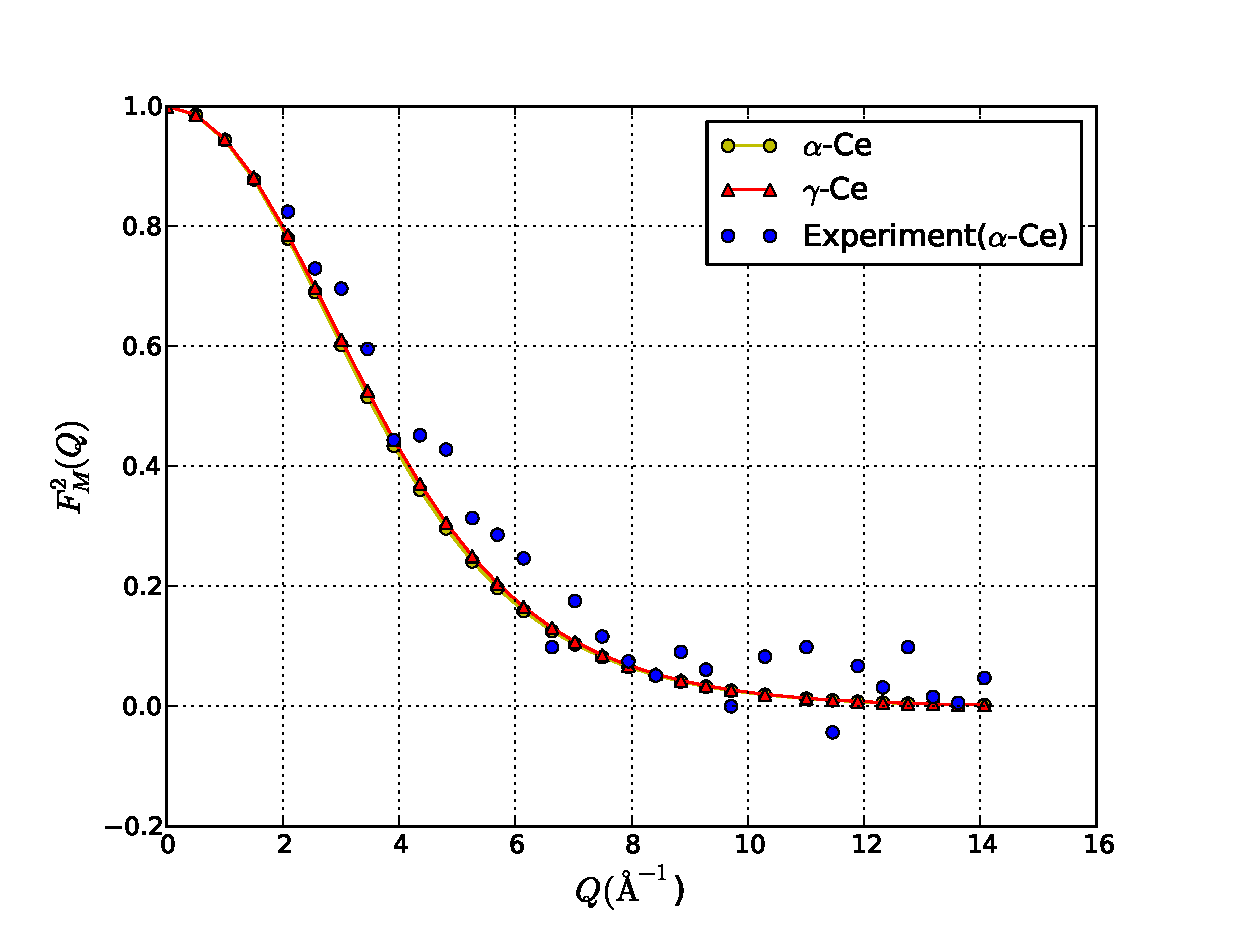
\includegraphics[width=0.99\linewidth,clip=]{Fig1.eps}
}
\caption{Momentum transfer dependence of the normalised magnetic form factor F$^2_M$(Q) of $\alpha$-Ce and $\gamma$-Ce. Blue circles show experimental data taken from Ref.\cite{murani}. 
}
\label{fig1_Ce}
\end{figure}
%


\subsubsection{Magnetic Form Factor}
The magnetic form factor $F_M(q)$ is the
Fourier transform of the spatial distribution of the electronic
magnetic moment, here mostly contributed by $4f$ electrons. Thus it is
an ideal observable for determining the nature of the $4f$ electrons.
In particular, the magnetic form factor can determine whether $4f$
electrons are localised or itinerant, as suggested in
Ref.\cite{hjelm1994}. The idea is the following: band formation
results in the quenching of the $4f$ magnetic moment, especially the
orbital component relative to the spin component. Thus, if the volume
collapse is due to a localisation-to-delocalisation transition, there
should be a dramatic change between the shape of the magnetic form
factor between the $\alpha$ and $\gamma$ phases.  For $\gamma$ cerium,
the measured magnetic form factor has free ion behavior, which is in
good agreement with the computed ionic Ce$^{3+}$ magnetic form
factor~\cite{stassis}.  On the other hand, for the $\alpha$ cerium,
electronic structure calculations predict metal-like behavior for the
magnetic form factor~\cite{hjelm1994}.  However, these calculations
are in striking contrast with recent high-energy neutron inelastic
measurements by Murani et al.~\cite{murani}, which show free ion
behaviour for the magnetic form factor of $\alpha$ cerium as well.


%
\begin{table}[!t]
\begin{tabular}{c|c|c}
 & $\alpha$-Ce & $\gamma$-Ce \\
 \hline
$\mu_s$ & $-2.3079\times10^{-3}$ & -0.03468 \\
$\mu_L$ & $9.3668\times10^{-3}$ & 0.13841\\
$C_2$ & 1.327 & 1.334 \\
\hline
 %$n_f$ & 0.91 & 1.00 \\
% \hline
 %$J_z^2 (a)$ & 3.21&2.76 \\
 %$J_z^2 (b)$ &3.24 &2.76 \\ 
\end{tabular}
\caption{
Values of the orbital ($\mu_L$) and spin $\mu_S$ magnetic moment as
obtained in our DFT+DMFT calculations under a magnetic field of 10T. The coefficient
$C_2=\mu_L/(\mu_L + \mu_S)$ determines the shape of the form factor in
the dipole approximation and has similar value in both phases.
%
% $n_f$ is the occupation number.$J_z^2 (b)$ denotes the value of calculated from L.H.S of sum rule check while $J_z^2 (a)$ denotes the values obtained from the actual impurity solver 
}
\label{table1_Ce}
\end{table}
%

Following the formalism described in Ref.\cite{mariettaMFF}, we
compute the magnetic form factor within the DFT+DMFT framework.
Figure~\ref{fig1_Ce} shows the magnetic form factor squared $F_M^{2}(q)$
in presence of an external magnetic field for both $\alpha$ and
$\gamma$ cerium.  The curves are close to each other and display free
ion behavior, typical of a correlated state. This is a consequence of
the electron-electron Coulomb repulsion, and cannot be captured solely
by electronic band structure effects. Our results are in good
agreement with the measured magnetic form factor of $\alpha$ cerium of
Ref.~\cite{murani}, and show that electronic structure calculations,
when combined with the dynamical mean-field theory, have the
predictive power to capture the magnetic response of the $4f$
electrons, and therefore to reconcile theory and neutron scattering
experiment.

To gain a deeper understanding of these results, we resort to dipole
approximation, $F_M = \mu (\langle j_0 \rangle + C_2
\langle j_2 \rangle)$, where $\langle j_k \rangle = \int dr\; u(r)
J_k(qr)$ is the spatial average of the spherical Bessel function
$J_k(qr)$ over the atomic cerium wave function $u(r)$,
$\mu=\mu_S+\mu_L$ is the total (spin plus orbital) magnetic moment,
and $C_2 = \mu_L/(\mu_S + \mu_L)$.  As shown in Table~\ref{table1_Ce},
$\mu_L$ and $\mu_S$ have opposite sign because of third atomic Hund's
rule (that is because of spin-orbit coupling and $n_f<1$), and
$\mu_L>\mu_S$, thus $C_2>0$.  The coefficient $C_2$ determines the
shape of $F_M(q)$ and remains basically unchanged across the
$\alpha-\gamma$ transition. It is close to the one expected for a free
Ce$^{3+}$ ion, implying that there is a localised $4f$ electronic
density for both $\alpha$ and $\gamma$ cerium.
%Table~\ref{table1} also shows that the occupation number $n_f$ decreases in the $\alpha$ cerium, in agreement with recent resonant inelastic X-ray scattering experiments~\cite{lipp2012}. 





%
\begin{figure}[!t]
\centering{
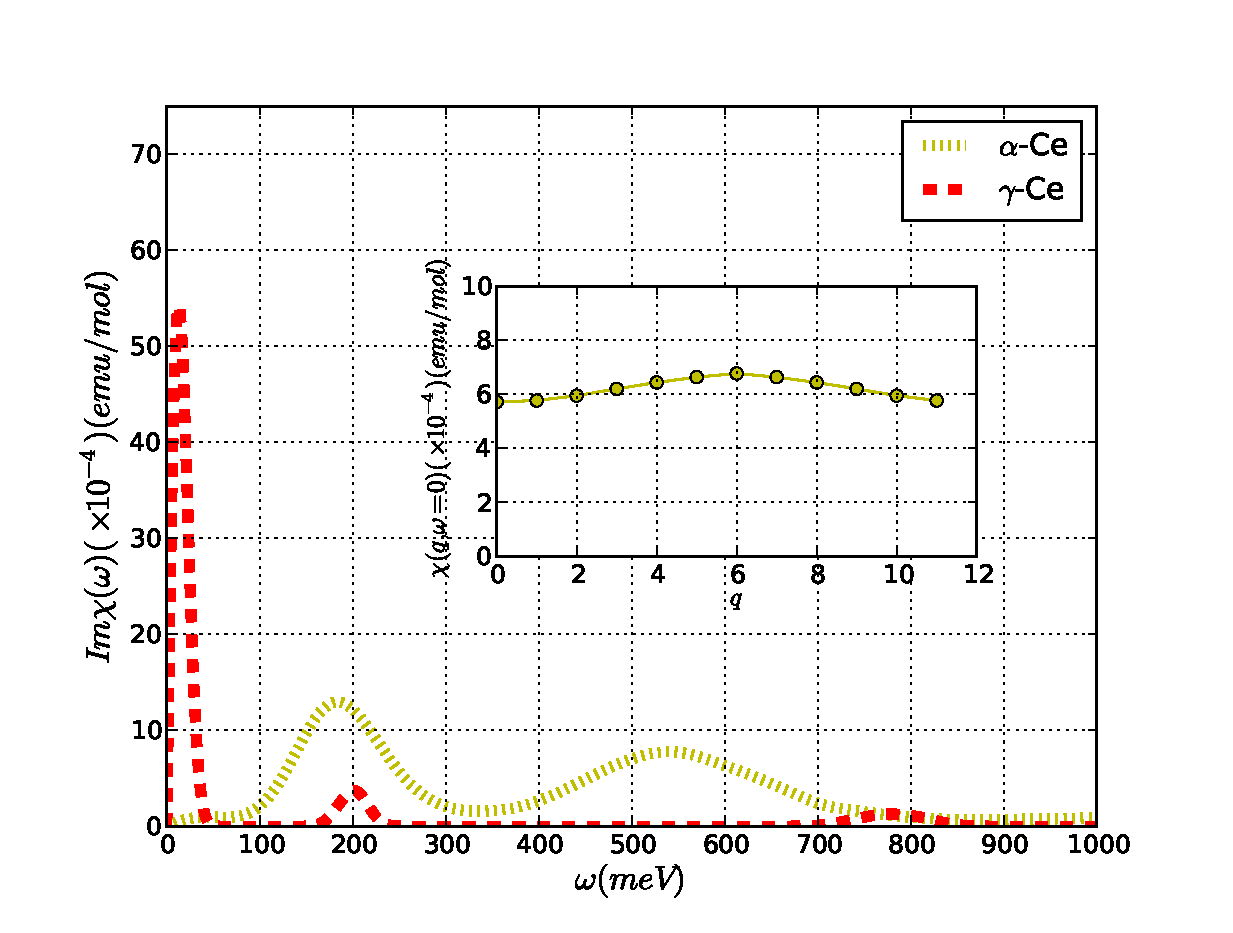
\includegraphics[width=0.99\linewidth,clip=]{Fig2.eps}
}
\caption{
  Imaginary part of the local dynamic magnetic susceptibility,
  Im$\chi(\omega)$, for $\alpha$ and $\gamma$ cerium (yellow dotted and red dashed lines  respectively). The inset shows the static
  susceptibility $\chi(q, \omega=0)$ of $\alpha$ cerium as a function of $q$ in the first Brillouin zone. Note that
  the $q$ goes from the points (0,0,0) to (1,1,-1) in 12 uniform
  steps.
}
\label{Susc_both}
\end{figure}
%
\subsubsection{ Dynamic Magnetic Susceptibility}
The magnetic form factor indicates that both $\alpha$ and $\gamma$ phase are strongly
correlated phases, which is compatible with both Mott and Kondo volume
collapse scenarios, but eliminates the promotional model.  In the Mott
scenario, the two phases are correlated because they lie on slightly
opposite sides of the delocalisation-localisation transition, while in
the Kondo volume collapse picture, the two phases are correlated
because the $4f$ electron moment remains stable across the transition.
However, the Kondo
volume collapse scenario differs from the Mott scenario because it
does not consider the $spd$ electrons to be mere bystanders, but
emphasizes their role in the screening of the local magnetic moments,
via the Kondo effect.  Therefore, the dynamic magnetic susceptibility,
which measures the spatial and temporal distribution of the magnetic
fluctuations, can indicate whether the hybridization plays a key role
at the transition.

In our calculations, we used the CTQMC impurity solver to obtain the
local dynamic  susceptibility $\chi(i\omega_n)$ of $\alpha$ and
$\gamma$ cerium as a function of Matsubara frequencies.  We then
analytically continued the data using maximum entropy method to obtain
Im $\chi (\omega)$ along the real frequency axis.  In Figure
\ref{Susc_both} we show Im $\chi(\omega)$ for both phases.  At small
frequencies, Im $\chi (\omega)$ for $\gamma$ cerium shows a narrow and
intense magnetic peak centered at approximately 10 meV. This feature
has to be expected from the local moment character of electrons in
$\gamma$ cerium.  The position of this peak gives a measure of the
Kondo temperature $T_K$.  For $\alpha$ cerium, this peak shifts to
higher frequency, around 180 meV.  Thus, in going from
$\gamma$ to $\alpha$ phase, there is a shift of magnetic intensity
from low to high energy, signalling a change (precisely, an increase)
in $T_K$.  This is one of the central results of our work.  We
emphasize that, at large frequencies, the overall intensity of Im
$\chi (\omega)$ in the $\alpha$ phase is larger than in the $\gamma$
phase, reflecting the increased hybridization of electrons in the
former phase.


In order to ascertain the nature of the different peaks in the dynamic
susceptibility of $\alpha$ cerium, we performed simulations of the
$\alpha$ phase with different values of spin-orbit coupling (not
shown).  Upon increasing spin-orbit coupling, the peak at low frequency
($\approx 180\,$meV) moves towards $\omega=0$.  This is a feature of
the fact that by increasing the spin-orbit coupling, the effective
Kondo temperature of the system is reduced.  Hence this peak is a
feature of the Kondo coherence energy of the system.  This trend has to
be expected because of the hybridisation between the conduction
electrons and the f electrons. By increasing the spin orbit coupling,
the energy splitting between the $5/2$ and $7/2$ states increases,
therefore fluctuations are hampered and $7/2$ states are less
occupied. It follows that the hybridisation with conduction electrons
decreases as well.  The importance of the spin-orbit coupling has also
been emphasized in the cerium compounds CeIn$_{3-x}$Sn$_x$ and
CePd$_3$~\cite{muraniSO, muraniCePd3, cox1987}.

The second peak ($\approx 600\,$meV) however does not show sensitivity
to the spin-orbit coupling.  To further ascertain the origin of the
second peak, we performed simulations with altered values of Hunds
Coupling $J$ (not shown).  The second peak is always roughly centred
at $\omega=J$ indicating that it represents an excitation of the the
f-electrons in the (non-zero) doubly occupied sector of f-electron
occupancy.

Notice that to crosscheck the validity of our analytic continuation
procedure, we benchmarked our results against a well-known sum rule
for Im$\chi(\omega)$. It is known that
$\dfrac{1}{\pi}\int_{-\infty}^{\infty} n(\omega)Im\chi(\omega) d\omega
= \langle \mu_{z}^{2} \rangle$ where $n(\omega)$ is the Bose
distribution function and $\mu_{z}$ is the magnetic moment along the z
axis, which can be independently extracted in our simulation without
need of analytic continuation.  A good quantitative agreement is
obtained in both phases.




In addition, we have verified that the local dynamical susceptibility
$\chi(\omega)$ is a good representative of the behavior of the
susceptibility $\chi(q,\omega)$ within the first Brillouin zone.  This
is important, because it verifies the so-called "single-ion form
factor dependence" often used to analize experimental
data~\cite{murani}, where the dynamical structure $S(q,\omega)$ is
factorized into momentum dependent form factor $F_M(q)^2$, and
energy dependent structure factor
$S(\omega)=\frac{1}{2}\frac{1}{1-e^{-\beta\hbar\omega}}$Im$\chi(\omega)$,
i.e, $S(q,\omega) = F_M(q)^2 S(\omega)$.  To verify the quality of
this approximation, we have computed the static susceptibility
$\chi(q, \omega=0)$ of $\alpha$ cerium within the first Brillouin zone
using a two particle vertex method, developed in
Ref.\cite{Park_prl11}.  We calculate $\chi(q)$ using the
Bethe-Salpeter equation $\chi(q)= (\chi_{0}^{-1}(q)-\Gamma)^{-1}$,
where $\Gamma$ is the two particle irreducible vertex, which we sample
within DMFT, and $\chi_0$ is the RPA susceptibility, which we compute
using the full k-dependent LDA+DMFT green's function. Note that within
DMFT, the two particle irreducible vertex $\Gamma$ is local. The inset
of Figure~\ref{Susc_both} shows $\chi(q, \omega=0)$. We can see that
there is no significant variation in the static susceptibility within
the first Brillouin zone, which validates the "single-ion form factor
formula".





\begin{figure}[t]
\centering{
\includegraphics[width=\columnwidth]{Sq_Ce.jpg}
}
\caption{Difference of $S(q,\omega)$ between $\alpha$ and $\gamma$ phase :
  Left panel shows DFT+DMFT  results. Right panel shows high energy neutron
  inelastic measurements, taken from Ref~\cite{murani}.
  }
\label{Sq}
\end{figure}
%%

\subsubsection{Magnetic  spectral Function $S(q,\omega)$}
  We then use this formula to
compute frequency dependent $S(q,\omega)$ of both phases.
Figure~\ref{Sq} shows the difference between the $\alpha$ and $\gamma$
magnetic spectral response ($S_\alpha(q,\omega)-S_\gamma(q,\omega)$).
In the lower panel we show the
experimental spectrum~\cite{murani}. There is a good agreement between
the two, particularly in the position of the broad peak assigned to
the Kondo screening in the $\alpha$-phase.  Note that the spectrum
displayed in Fig.~\ref{Sq} becomes negative in the low energy region
where $\gamma$-Ce susceptibility has sharp peak due to local moment character
(see Fig.~\ref{Susc_both}).  This region has been left out of
theoretical (as well as experimental) plot so as to enable better
visualization of the other features.
%Also note that the experiment is carried out at 140 K
% whereas we perform our simulations at 116 K.

\subsubsection{Conclusions} 
In summary, we showed theoretically that the neutron magnetic form
factor $F_M(q)$ has a free ion behaviour in both phases, indicating
that the $4f$ electrons remain strongly correlated across the
$\alpha$-$\gamma$ transition.  On the other hand, the local dynamical
susceptibility $\chi(\omega)$ and the magnetic spectrum $S(q,\omega)$
show dramatic changes across the transition, with an energy shift from
lower to higher frequencies, a direct consequence of the increase of
the Kondo temperature $T_K$ in the $\alpha$ cerium.  Therefore, our
data shows that the physics of the volume collapse $\alpha$-$\gamma$
transition in cerium is controlled by the hybridization between the
localised $4f$ and the $spd$ electrons and also establishes the
importance of using different probes and observables to understand
different aspects of the volume collapse transition in cerium.

\subsection{The valence fluctuating ground state of Plutonium}

\subsubsection{Introduction}

Plutonium (Pu) is well-known due to the radioactive instability of its nucleus which makes it an important material for nuclear fission. However, the electronic properties of Pu have also attracted a lot of attention due to the presence of multiple degenerate configurations due to it's position in the periodic table.Pu is an actinide and therefore has an incomplete 5f electronic shell.  among the first few members of the actinide series, there is a volume contraction which is observed with increasing atomic number, due to the excess screening provided by the comparatively delocalized nature of the 5f electrons being added . However in the last few members of the actinide series, one observes an increase in atomic volume with increasing $Z$ because at this point the 5f electrons are highly localized and do not screen the nuclear charge. Plutonium sits at the cusp of these two two different subgroups of Actinides and therefore has an exceeding complex electronic structure, which has been the subject of intense study for more than six decades. This complexity also manifests itself in the highly complex phase diagram exhibited by Pu, with six competing allotropic phases which unusually large volume differences between then of up to 25$\%$ accompanied by large variation in mechanical properties (see Fig \ref{Pu_phase}) . In this particular study we shall study the properties of the delta phase ($\delta$-Pu). 

\begin{figure}[H]
\begin{center}
\includegraphics[width=0.7\columnwidth]{Plutonium_phase_diagram.png}
\caption{The Volume vs Temperature Phase diagram for Plutonium showing the multiple phases of the material}
\label{Pu_phase}
\end{center}
\end{figure}

The face centered cubic (fcc) $\delta$-Pu displays Pauli-like magnetic susceptibility (like $\alpha$-Ce)  as well as an anomalously highly  Sommerfeld coefficient of the specific heat  due to its unique combination of itinerant and localized electronic states  \cite{Lashley1,Quint_1,Yang}, which makes it an extremely interesting problem to study in strongly correlated materials, far away from the well understood limits of completely itinerant or localized electronic structures . This inability to describe the exact electronic structure properties has resulted in a lot of disagreement between theory and experiment, with theories that can accurately predict the volume and structural fluctuations concurrent with the phase transitions exhibited by Pu being completely unable to reproduce the lack of a static magnetic moment, as is required by the Pauli-like susceptibility shown by $\delta$-Pu, and confirmed by experiments. This is known as the missing magnetism problem of $\delta$-Pu

However, this kind of electronic structure problem where there is an interplay between localization/delocalization is exactly the domain where DFT+DMFT comes into its own. In order to correctly capture the physics of this material, we need to preserve the quantum mechanical fluctuations present, which result in the material fluctuating between three different atomic valency states, namely $5f^4$ (Pu 4+), $5f^5$ (Pu 3+), and $5f^6$ (Pu 2+). Since we preserve all local quantum fluctuations in DFT+DMFT, we can accurately model these virtual valence fluctuations. An extremely sensitive and important tool to capture this effect is the magnetic spectral function $S(q,\omega)$, because the magnetic formfactor $F(q)$ displayed by $\delta$-Pu is markedly different than the one displayed by any calculations which neglect valence fluctuations. In addition, any accurate simulation of $S(q,\omega)$ would also have to be display a Pauli-like susceptibility which would rule out a static magnetic moment. In addition neutron scattering experiments, similar to Cerium, would provide an experimental verification of our theoretical predictions  . Plutonium being a radioactive element, performing experiments on it can be extremely difficult. However recently experiments were performed at Oak Ridge National Labs which gave verified our calculations and which were published in Ref \cite{Me_Pu}. We shall present the results below but for more details the reader should refer to the reference.


\subsubsection{Details of Method}

In our calculations, we performed  DFT+DMFT calculations with a Hubbard U of $4.5$ eV and a Hunds J $0.512$ eV. All calculations were performed at an electronic temperature of 232 Kelvin. As noted earlier for calculations of the magnetic formfactor we have to use the NCA impurity solver due to the sign problem faced by CTQMC in the presence of off-diagonal hybridization introduced by the magnetic field used in formfactor calculations.For calculations of the magnetic susceptibility, we used CTQMC. In order to obtain highly converged converged results, simulations were performed on the Titan supercomputer at Oak RIdge National Lab. Of the order of 500 DFT and 30 DMFT cycles (totalling 10 million core hours) were used for high quality runs, which can be analytically continued to real frequencies using maximum entropy. Spin orbit corrections were incorporated in all the simulations since spin-orbit corrections are very important in 5f materials.

\subsubsection{Magnetic Formfactor}

\begin{figure}[H]
\begin{center}
\includegraphics[scale=0.5]{Formfactor_Pu.jpg}
\caption{The DMFT Formfactor obtained by our simulations for $\delta$-Pu, together with neutron scattering results at 250 and 500 meV incident neutron energies and the formfactors that would have been obtained by considering a pure $5f^4$ or $5f^5$ valence, as well as a admixture of the two}
\label{Form_Pu}
\end{center}
\end{figure}

The magnetic formfactor obtained by us is shown in Fig \ref{Form_Pu} (taken from our published paper \cite{Me_Pu}). The figure also provides the experimentally obtained formfactor and the formfactors that would have been obtained by considering a pure $5f^4$ or $5f^5$ valence, as well as a admixture of the two that is empirically close to the experimental results. As we see, DMFT is successful is capturing the correct form of the formfactor. We see that the $5f^5$ formfactor is also a reasonable fit with experiment. However a pure $5f^5$ state would have a magnetic moment and is hence not suitable to reproduce the Pauli-like suceptibility we observe. It is to be noted that at low Q, the experimental errors are very large due to experimental limitations. Therefore the discrepancies with experiment are not considered very relevant . However we clearly see that DFT+DMFT is successful in capturing the correct spatial dependence of $S(q,\omega)$ through the magnetic formfactor. 


\subsubsection{Dynamic Suceptibility and $S(q,\omega)$}

\begin{figure}[H]
\begin{center}
\includegraphics[scale=0.5]{Susc_pu_cropped.jpg}
\caption{ The Imaginary part of the local dynamic susceptibility for $\delta$-Pu compared to neutron scattering experiment \cite{Me_Pu} }
\label{Susc_Pu}
\end{center}
\end{figure}

The dynamic magnetic susceptibility calculated for $\delta$-Pu is given in Fig 6.7. In the figure, we also see the experimental results from \cite{Me_Pu} (the actual reference contains multiple experimental results ommitted here for clarity). As we see, DMFT is able to capture the correct location of the peak in the dynamic susceptibilty at ~84 meV, which gives us the relevant scale for spin excitations. It is to be noted that these results predict a Kondo Temperature of $\sim$800 K (in agreement with results obtained by Haule et. al \cite{Haule_Pu} )  which explains why at room temperature the moment of the 5f state is screened by the Kondo screening cloud of antiparallely alligned conduction electrons , which screen the magnetic moment. By using the sum rule in Eq. \ref{sum rule} we obtain a fluctuating moment of $\sim$ 0.8 $\mu_B$ per atom which is also in good agreement with experiment. Finally we note that for any static local moment phase, we would have seen a Curie-like susceptibility which is characterized by a peak in the imaginary part of $\chi(\omega)$ at very low frequencies, analogous to $\gamma$-Cerium. However no such peak is observed. Therefore we can see that we have no local moment behaviour in this material


\begin{figure}[H]
\begin{center}
\includegraphics[width=\columnwidth]{Sq_Pu_joined.jpg}
\caption{ The Magnetic Spectral Function $S(q,\omega)$  for $\delta$-Pu compared to neutron scattering experiment \cite{Me_Pu}. The dashed lines on the experimental figure denote the Q and $\omega$ values used to obtain the formfactor and the Susceptibility. The peak position corresponding to $k_B T_K$ is also marked \label{Sq_Pu_fig} }
\end{center}

\end{figure}

Finally we show in Fig 6.8 the $S(q,\omega)$ for $\delta$-Pu using DFT+DMFT as well as by neutron scattering. As we can see (and as can be expected from the fact that both the formfactor and the susceptibility are in good agreement with experiment) we can very good agreement between theory and experiment. Therefore we can claim that using DFT+DMFT, we can obtain an exceedingly accurate description of the magnetic spectrum of $\delta$-Pu and get very important clues which shall help us in understanding the true nature of this compound.

Therefore in conclusion, we have shown that we have developed a robust method to calculate the magnetic spectrum of correlated systems. We have used our method to understand the magnetic structure of both Cerium and Plutonium and have obtained very accurate experimentally verifiable results. Therefore we believe that in the future we can use our method to understand the magnetic properties of a large class of strongly correlated systems.


\pagebreak
\chapter{Spin State Transition in $\mathbf{LaCoO_3}$}

\section{Introduction}
The spin state transition in LaCoO$_3$ has been the subject of  intensive investigation for decades.\cite{Heikes, Naiman, Goodenough}.At low temperature, this compound is known to be a to be a narrow bandgap insulator  with Pauli-like magnetic susceptibility. However between 90-150 K, it transitions to a local moment phase with a Curie-Weiss like susceptibility which reaches its peak around 150K. It also undergoes a gradual closing of the insulating gap and is known to be metallic above 600K \cite{BhideMoss, English, Saitoh}.

There is considerable debate regarding the mechanism of this transition, mainly due to the uncertainty regarding the multiplet of the $Co^{3+}$ ion which  characterizes the excited state of the compound.  The cobalt ion in LaCoO$_3$ is commonly considered to have a formal valence of $3+$ and to be in the $d^6$ state. The scale of the crystal field splitting is comparable to the Hunds coupling energy scale. As a result, one would expect that as temperature is increased, there would be an entropy-driven transition from the low spin (LS) $S=0$ state with a fully filled $t_{2g}$ shell($t^6e^0$) to an $S=2$ high spin (HS) state ($t^4e^2$)\cite{Goodenough}. Indeed there is experimental evidence to support such a scenerio. Electron spin resonance\cite{Zopka}, neutron scattering \cite{Podlesnyak}, X-ray absorbtion spectroscopy and magnetic circular dichroism experiments\cite{Haverfort} point towards a transition to an HS state. In addition, no inequivalent Co-O bond is found in EXAFS experiements, which also supports the formation of an HS state due to the HS state not being strongly Jahn-Teller active \cite{Sundaram}. However, it has been noted that in order to explain the  XAS experimental data, one would have to assume that the crystal field grows with temperature, which is counter-intuitive.\cite{Eder, Haverfort} This led to some authors suggesting that there is an LS-HS alternating structure , which forms as a result of by breathing distortions in the lattice \cite{Bari} \cite{Goodenough} and interatomic repulsion between the HS atoms.\cite{Asaka, Eder} 
 
A competing explanation, whereby the excited state is the $S=1$ intermediate spin (IS) state ($t^5e^1$), has also become popular\cite{Heikes, Radaelli}, mainly because of LDA+U results which show that the    
IS state is lower in energy compared to the HS state.\cite{Korotin, Pandey, Anisimov} The stability of the IS state has been justified by the large hybridization of the Co 3d electrons with neighboring O 2p electrons. This causes charge transfer between the ions resulting in the Co ion having a $d^7$ structure according to the Zaanen-Sawatzky-Allen scheme,\cite{Zaanen} which in turn would cause stabilization of the IS state. The intermediate spin state hypothesis also seems to explain experimental findings such as Raman Spectroscopy, X-Ray photoemission, other XAS and EELS spectroscopies, as well as susceptibility and thermal expansion measurements. \cite{Saitoh, Abbate, Masuda, Klie, Zobel, Gne, Maris, Vogt}. 

To summarize, there has been significant debate regarding the true nature of the spin state transition in LaCoO$_3$ (see Fig \ref{Transition}). Interest in this compound has also been enhanced in light of recent discoveries of ferromagnetism induced by Sr (hole) doping \cite{Kriener, Masayuki, Kunes_doped,nemeth}, as well as experiments reporting strain induced magnetism in epitaxially grown thin films.\cite{Fuchs1, Fuchs2, Rondinelli, Freeland, Fuchs3, Herklotz,Hsu}.Additionally, there have been reports of the emergence of a striped phase in thin films with alternating LS and HS/IS regions.\cite{Striped}   Low temperature ferromagnetism has also been reported in experiments on $LaCoO_3$ nanoparticles\cite{Belanger1}. Hence, there is great interest in understanding the true behavior of this material. 

 \begin{figure}[H]
 \begin{center}
 \includegraphics[width=\columnwidth]{Transition_figure.jpg}
 \caption{Schematic illustration of the two different scenarios for the the spin state transition in LaCoO$_3$ }
\label{Transition}
 \end{center}
 \end{figure}
 
In this chapter, we use Density Functional Theory + embedded Dynamical Mean Field Theory (DFT+DMFT)  to analyze the spin state transition of bulk $LaCoO_3$.  Our implementation extremizes the DFT+DMFT functional in real space, thereby avoiding the downfolding approximation and uses the numerically exact CTQMC impurity solver\cite{Dmft3,haule}.  Even though there are multiple recent studies that use DFT+DMFT on this compound \cite{craco, Zhang, Kunes_main}, to our knowledge none of them provide a comprehensive analysis of all of the factors governing the transition such as octahedral rotations and electronic entropy. We show that i) LaCoO$_3$ has large charge fluctuations and it is not possible to explain the spin state with a single multiplet at any temperature, ii) The crystal field splitting very sensitively depends on the details of the crystal structure, and taking into account not only the thermal expansion but also the oxygen octahedral rotations is very important, and  iii) It is possible to stabilize an insulating phase (without orbital order) at intermediate temperatures where local moments are present, thereby showing that the metal-insulator transition is distinct from the spin state transition in this compound. We also show that  iv) Electronic entropy difference between the high and low temperature states is necessary for the stabilization of the different spin states, which is a fact overlooked in various first principle studies so far. 


\section{Crystal Structure of LaCoO$_3$}

LaCoO$_3$ is a perovskite, which has the rare earth La on the A-site and Co on the B-site   , which corresponds to the center of the oxygen octahedron (see Fig \ref{Perov_struct}). However, like most of the perovskites, LaCoO$_3$ has oxygen octahedral rotations (Fig. \ref{structure}) which involves the oxygen octahedra rotating out-of-phase around the [111] axes of the undistorted cubic highsymmetry structure. The rotation pattern in Glazer notation is $a^-a^-a^-$, which corresponds to the space group R$\bar 3$c (\#167).

\begin{figure}[H]
 \begin{center}
 \includegraphics[height=4in]{plots_final/supplement_plots/perovskite_struct}
 \caption{Conventional cell for a perovskite with no octahedral rotations ($a^0a^0a^0$ structure). In LaCoO$_3$, the green atoms would be 
La, the red atoms O and the blue atom Co. The figure also shows the octahedra formed by the oxygen atoms around the Co atom}\label{Perov_struct}
\end{center}
\end{figure}


As noted by Thornton et. al. \cite{Thornton}, LaCoO$_3$ has large thermal expansion and the octahedral rotation angle also changes with temperature. In our study, we used four different crystal structures to isolate and study the effect of different lattice parameters on the spin state transition. We used the two different experimental structures observed at 1143K and 4K, which we denote by $HTa^-$ and $LTa^-$. Comparing the electronic structure for these two crystal structures provides a means to study the temperature evolution of the electronic structure. In addition to these two, we also built two crystal structures with the same strain state (unit cell vectors) as them, but with no octahedral rotations. These structures, denoted by $HTa^0$ and $LTa^0$, enabled us to isolate the effect of oxygen octahedral rotations on the strain state of LaCoO$_3$. 

\begin{figure}[H]
 \begin{center}
 \includegraphics[height=4in]{plots_final/supplement_plots/a-a-a-_struct}
 \caption{A depiction of the pattern of octahedral rotations that is present in LaCoO$_3$. Each of the oxygen octadra rotates in opposite direction to all nearest neighbour octahedra by the same amount relative to all three coordinate axes ($a^-a^-a^-$ structure).}\label{structure}
 \end{center}
 \end{figure}






In Fig \ref{LaCoO3_dos} we show the density of states for all 4 structures, calculated at both low temperature and high temperature (116K and 1160K) using DFT+DMFT. Unlike DFT, which always predicts a metallic state, our calculations correctly reproduce an insulating ground state at low temperature for all the structures. The $t_{2g}$ orbitals are below the fermi level whereas the $e_g$ orbitals are above the fermi level. 

\begin{figure}[H]
\begin{center}
\includegraphics[width=\columnwidth]{plots_final/output/New_Dos.png}
\caption{Density of states ($t_2g$,$e_g$ and total including all atoms) for all four structures at 116K and 1160K.}\label{LaCoO3_dos}
\end{center}
\end{figure}

The charge gap closes continuously with increasing temperature, and as a result, there is a large overlap in energy between the $t_{2g}$ and $e_g$ orbitals at high temperatures. This overlap, however, is much smaller if the structures without rotations are simulated. (See Fig. 2b).

The $HTa^0$ structure  shows some overlap at high temperatures, and the $LTa^0$ structure almost remains an insulator for the entire range of temperature studied, with a small overlap developing above 900K. 
%
This shows clearly that octahedral rotations play a large role in decreasing the strength of the crystal field splitting. 
This can be explained by a combination of factors. The rotation of the oxygen octahedra causes misalignment of the crystal field of the O atoms with that of the La atoms, which normally reinforce each other in a  perovskite with no octahedral rotations. This leads to an overall reduction of the effective crystal field which reduces the charge gap between the $t_{2g}$ and $e_g$ orbitals. In addition, this trigonal distortion also leads to a splitting of the $t_{2g}$ orbitals into 2+1 orbitals, thereby again reducing the gap with the $e_g$ orbitals (Note that in Fig \ref{LaCoO3_dos} we have clubbed together all of the 2+1 orbitals into one single "$t_{2g}$" group because the splitting is small compared to the $t_{2g}-e_g$ splitting  and doing so makes the figure clearer). The combination of these two effects seems to overcome the expected decrease in the bandwith of the $e_g$ orbitals caused by the bending of the Co-O-Co bond.Finally, note that there is a considerable overlap in energy of the O 2p orbitals with the Co 3d orbitals, which is very important in producing charge fluctuations on the Co ion, making it highly mixed-valent. 


\begin{figure}
\begin{center}
\includegraphics[width=\columnwidth]{plots_final/output/fig2.png}
\caption{(a) Evolution of $|S_z|$ with temperature for all four structures. (b) Evolution of Density of states at fermi level with temperature for all four structures.}
\end{center}
\end{figure}

\section{The spin state transition} 
In order to focus on the spin state of the Co ion, we calculate the expectation value of the magnitude of z-component of the spin $\langle|S_z|\rangle$. Note that all our calculations are in the paramagnetic state and hence the value of $\langle S_z \rangle=0$. The results are presented in Fig. 2a as a function of temperature. Note that the quantitative value of the transition temperature is overestimated in our calculations. This can be explained by the fact that DMFT does not take into account finite wavelength fluctuations, and as a result, has a tendency to overestimate order like many other mean field methods.
The largest value of $|S_z|$ at 1160K is seen for the $HTa^-$ structure, followed by the $LTa^-$ structure. 
%
This is in line with the stronger crystal field in the $LTa^-$ structure due to the smaller lattice constant.
We also observe that  the spin state transition starts at a higher temperature for the $LTa^-$ structure ($\sim$580K) compared to the the $HTa^-$ ($\sim$380K). This is also consistent with the the low temperature structure having higher stability for the LS state. 
The structures without rotations consistently show lower buildup of higher spin states than the ones with rotations. The $HTa^0$ structure displays a spin state transition, but with an eventual high temperature value of $|S_z|$ that is lower. On the other hand, the $LTa^0$ structure shows almost no transition. This shows that the role that the octahedral rotations play in the reduction of the crystal field is essential for the spin state transition.

Figures 2a and 2b also show that the spin state transition and the charge gap closing occur at different temperatures, which is a trend that has been observed in experiment but has not been captured in earlier DMFT simulations. For example, Fig 2b shows that both the $HTa^-$ and the $LTa^-$ structures show a complete closure of the charge gap at $\sim$ 600K whereas Fig 2a shows that the spin state transition in the two structures occur at very different temperatures. 



\section{Nature of the excited spin state}
 Because of the large hybridization between Co and O, the d orbitals of Co have large charge fluctuations and all the four structures have an effective d-shell occupation of $n_d \sim 6.6$. Therefore any analysis of the spin states in terms of the LS, IS and HS states of the $d^6$ configuration of the Co ion is necessarily inadequate. In fact, our calculations show that the $d^7$ configuration has a higher occupation probability than $d^6$, and there are also significant probabilities for $d^5$ and $d^8$

Fig. 3 shows the evolution of the occupation probabilities for the different values of $|S_z|$ with temperature. Even at high temperatures, $|Sz|=0$ and $|S_z|=0.5$ (the LS states for the even and odd occupancy sectors of the d orbital) remain the states with the highest probability. However, with the increase of temperature, the weight of the higher spin states increases. 
%
 At the onset of the transition, the initial change in the value of the spin state is predominantly caused by the excitation of the $|S_z|=2$ and the $|S_z|=1.5$ multiplets.  
The $|S_z|=1$ multiplet sees an increase in probability at higher temperatures (above 500K) and also follows a similar trend for all the structures except the $LTa^0$ structure, where all changes are very small. Therefore, the initial signature of the transition is best seen in the behavior of the $|S_z|=2.0$ and $|S_z|=1.5$ multiplets, which can be said to be the HS multiplets for the $d^6$ and $d^7$ occupancies respectively. 
 \begin{figure}
 \begin{center}
 \includegraphics[width=0.7 \columnwidth]{./plots_final/output/New_Sz.png}
 \caption{Evolution of occupation probabilities for all the spin states for the four structures with temperature. }
 \end{center}
 \end{figure}


\begin{figure}
\includegraphics[width=\columnwidth]{./plots_final/output/hist_final.png}
\caption{Occupancy histogram showing the occupancy Probability for the different atomic states for the d orbital of the Co atom for all the four structures at two different temperatures. The different background colors mark the areas reserved for different spin sectors.  The lower x axis ticks as well as the color of the histogram bars denote the different occupancies of the d orbital. Note that odd occupancies only allow half integer values of $|S_z|$ while even ones allow integer values}
\end{figure}


In Fig. 4, we show the occupancy histograms below and above the transition (at 116K and 1160K).(CTQMC gives us access to the state space probability for each of the 1024 states of the d orbital. However, in order to aid visualization, we only show states which have an occupation probability above 0.001 in any of the structures at any temperature.) This figure displays clearly how the transition is marked by the excitation of states in the higher spin multiplets. We see that the low temperature state for all of the structures is marked by the presence of a few states with large probability (mainly corresponding to the $|S_z|=0$ and $|S_z|=0.5$ states). As the spin state transition sets in, a large number of higher spin states get excited and the LS spin states lose weight. Note that the high spin states are highly degenerate so there is no one large peak for the high spin states, but a multitude of lower peaks. This supports the idea that the transition is primarily an entropy driven transition. We can also get a good idea of the relative strengths of the transition for the different structures: The largest change occurs in the $HTa^-$ structure, and the smallest one happens in the $LTa^0$. 

\section{Contribution of Electronic Entropy} 
According to the entropy driven transition scenerio, which is supported by calorimetric measurements\cite{Stolen}, LaCoO$_3$ favors higher spin multiplets  at elevated temperatures because of the  associated gain in electronic entropy as a result of the high degeneracy of these high spin states - a point missed by first principles calculations at the level of DFT. Access to higher spin states is also made easier by a larger lattice constant due to the reduced crystal field, so the gain in electronic entropy could also be a driving factor for the large thermal expansion seen in this material.

We calculated the contribution of the electronic entropy to the free energy using our state of the art DFT+DMFT implementation\cite{Birol}. 
In particular, we evaluated the Free Energy and the Electronic Entropy for both the 4K and 1143K structures ($LTa^-$ and $HTa^-$) at 1160K to predict if the structural changes make a considerable difference. 
%
The $HTa^-$ structure is indeed much higher in electronic entropy compared to the $LTa^-$ structure at 1160K; the difference in $T\cdot S$ between these two structures is $\sim$ 110 meV per formula unit. This unusually large difference emphasises the importance of electronic entropy to the transition.We also calculate the energy difference between the $HTa^-$ and $LTa^-$ structures to be $\sim$ 70meV at 1160K with the $LTa^-$ being lower in energy. Thus we see that when the entropy is taken into account and the Free Energy (F=E-TS) is calculated, the high temperature structure $HTa^-$ becomes more stable purely due to the contribution of electronic entropy (see Fig \ref{Entropy_Swap}).  This result therefore confirms the structural phase transition that is observed as a function of temperature. So, we can conclude that the electronic entropy, which has been ignored in many first-principles studies of this material, is a leading factor in creating an anomalous thermal expansion and driving the material to a high spin state. 
\begin{figure}[H]
 \begin{center}
 \includegraphics[width=\columnwidth]{Entropy_swap.jpg}
 \caption{A depiction of the Switch in stability between the $LTa^-$ and $HTa^-$  structures due to the impact of electronic entropy.}\label{Entropy_Swap}
 \end{center}
 \end{figure}



\section{Summary} 
We studied the spin state transition of LaCoO$_3$ using state of the art fully charge self consistent DFT+DMFT. By using different experimental and hypothetical crystal structures, we disentangled the effect of different components of the crystal structure and showed that both the thermal expansion and the presence of oxygen octahedral rotations have tremendous effect on the spin state transition of LaCoO$_3$. Our single site DMFT approach reproduced not only the spin state transition but also the intermediate phase which has nonzero magnetic moment but is insulating. This shows that the spin state and the metal-insulator transitions occur at different temperature scales and that the magnetic-insulating phase can be reproduced without  necessarily involving cell doubling via mechanisms such as breathing distortions of spatially inhomogenous mixed spin states. Our results emphasize the importance of charge fluctuations on the Co ion due to hybridization with the O anions, and thus point to the inadequacy of a simple spin state picture with only one formal valence. While the spin state transition is concurrent with a sudden change in occupation in the high spin multiplets, low and intermediate spin states also have significant occupation in the whole temperature range. Finally, our work is the first calculation of the electronic entropy of LaCoO$_3$ and it points to the fact that the difference of the contribution of entropy to the free energy is significant and is large enough to drive the spin state transition in this material. 

\pagebreak
\chapter{Investigation into the inadequacy of cRPA in reproducing screening in strongly correlated systems}
\section{Introduction}
 Achieving a truly \emph{ab initio} description of  materials with strongly correlated electrons is one of the prime objectives of condensed matter physics today.These compounds attract interest as they often have very complicated phase diagrams displaying a variety of interesting phenomena such as  metal- Mott insulating transition(MIT), unconventional superconductivity and non-trivial magnetic order,charge/spin density waves etc\cite{RMP_MIT_1998_Imada}. These phenomena cannot be explained by free electron-based approximations and often lie beyond the scope of density functional theory(DFT),the workhorse for predicting properties of solids from first principles\cite{RMP_dft_review_1989_R_O_Jones}. Dynamical Mean Field Theory (DMFT) seeks to overcome some of the difficulties of studying these systems by mapping the lattice problem to a numerically tractable auxiliary impurity problem coupled to a bath which is determined self-consistently. This approach, which was originally created to study model hamiltonians such as the Hubbard model, has recently been combined with DFT (DFT+DMFT) and has proved to be highly successful in explaining the properties of strongly correlated materials \cite{RMP_LDA+DMFT_2006_G.K}.Various implementations of DFT+DMFT are currently available\cite{PRB_Wannier_Downfolding_2006_D.Vollhardt,PRB_Wannier_Downfolding_2006_O.K.Andersen,PRB_localorbital_Downfolding_2008_Lichtenstein,PRB_dmft_wien2k_2010_Chuck_Haule,PRB_LaFeAsO_2010_A.Georges,PRB_covalency_TMoxides_2014_k.Haule},which mainly differ in i)the choice of how to project to the localized impurity degrees of freedom and ii)the energy window used while embedding the impurity self-energy into the DFT lattice eigensystem .Though the relative merits of a particular scheme might be dependent on the problem at hand, a common issue facing all of them is the determination of the material-specific effective interaction parameters like the Hubbard $U$ and Hunds $J$ for the correlated subspace. The lack of a reliable prediction procedure is one of the primary reasons this method cannot yet be considered truly \emph{ab initio}.

This well-known problem was pointed out soon after the introduction of the Hubbard model and early attempts to estimate the Hubbard $U$ in real materials were made by Cox et.al \cite{IOP_HubbU_transition_metal_1973_B_N_Cox}. Subsequent advances led to development of a method based on the Local Density Approximation(LDA) called cLDA (constrained LDA),  in which the Hubbard $U$ is calculated from the energy difference between different occupations of the localized orbitals after cutting off all hopping from the correlated orbitals to the itinerant states\cite{PRB_cLDA_Cuprates_1988_McMahan,PRB_cLDA_cuprates_1989_Christensen,PRB_cLDA_Fe_Ce_1991_Anisirnov}.
However, this method tends to overestimate $U$ since a lot of physical screening channels are eliminated when the hoppings are cut off. 
%There have been attempts to improve cLDA by incorporating linear response \cite{PRB_linear_response_2005_Gironcoli}. 
Recently, another  approach based on the Random Phase Approximation(RPA) called constrained RPA (cRPA)\cite{PRB_CRPAMethodInvented_1998_F.Ary,PRB_lowenegymodel_for_firstprincilpes__2004_F.Ary} has  gained popularity as it is material-specific and provides a clear picture of the physical screening channels which are taken into account.  cRPA has been applied to a variety of strongly correlated systems such as transition metals and their oxides\cite{PRB_CalculationofHubU_cRPA._2006_F.Ary,PRB_cRPAonTransitionMetal_2008_F.ARy,PRB_cRPAonTransition_oxide_2012_S.Biermann,PRB_cRPAonTransition_oxide_2012_P.H.Zhang,PRB_cRPAonTrans_oxides_2013_F.Ary},early lanthanides\cite{PRB_cRPAonearlyLanthanide_2013_F.Ary,PRB_Screened_Coul_inter_cal_2014_F.Bruneval} and high-Tc superconductors\cite{JPSJ_lowenergyOFironbaseSC_2010_M.Imada,PRB_DyanmicScreening_LaCuO_2015_P.Werner_F.Ary}. However,the Hubbard $U$ predicted by cRPA is generally not in good agreement with the value required by DMFT impurity solvers to achieve agreement with experiment. One notable example \cite{PRB_Screened_Coul_inter_cal_2014_F.Bruneval} is elemental Cerium for which the $U$ predicted by cRPA is about 1eV, which is far smaller than the value of around 6eV used in practice . 
This is not surprising since the Ce $f$ orbital is more localized than the transition elements' $d$ orbital and cRPA is suspected to be inadequate for such strongly correlated systems. In spite of this, there has been little theoretical investigation into exactly why cRPA fails in the strongly correlated regime. Instead  most of the recent research on cRPA has focused on the energy window to be used in the cRPA procedure and the definition of the many-body model using the effective  $U$ predicted by cRPA \cite{PRB_cRPAonTrans_oxides_2013_F.Ary,JPSJ_lowenergyOFironbaseSC_2010_M.Imada}. In view of the above, we firmly believe that further investigation is required into the root causes of the failure of this method when strong correlations are present. 

In this paper,we investigate the accuracy of cRPA using a class of model Hamiltonians based on models used to study strongly correlated materials. This allows us to  study the fundamental causes for the failure of cRPA in strongly correlated systems in general, instead of merely making predictions about a specific compound. %It is known that cRPA works(not very sure...) in the case that the screening bands are far away from the low-lying bands\textbf{If so, put a reference}.
In all of our models, we include strong hybridization between localized and itinerant bands as the accuracy of cRPA is particularly questionable in such systems. Our models are two dimensional and we retain all density-density Hubbard interactions, reminiscent of the models used to study typical transitional metal oxides. 
%I thought these hamiltonians were used to study Cuprates, not generic transition metal oxides! 
We use DMFT to compute the spectra and quasiparticle residues of both the full multi-orbital model as well the effective one-orbital model using parameters obtained from cRPA. We show that \textrm{i)} cRPA has a tendency to systematically overestimate screening in the system. \textrm{ii)} We also find that for a large range of parameters, inter-orbital and weakly correlated orbitals' U parameters have little effect on the spectrum, thus negating the fundamental screening mechanisms used in cRPA. \textrm{iii}) Instead, we study a far more accurate form of W and U using the DMFT local Polarization bubble which exactly includes all local interactions. Using this new method, we show that the true screening is far less than predicted by cRPA/RPA and that the actual U predicted by this method has little frequency dependence. \textrm{iv)} We also study the fully screened interaction(W) evaluated using RPA and our new method and show that the RPA W is unable to capture the Mott transition and also shows no signatures of local screening processes, which are present in in the W evaluated using our new method. Since local interactions are treated exactly in DMFT, this success of the local Polarization method clearly shows that DMFT takes into account all the predominant screening processes in strongly correlated systems which are missing from RPA-based approaches. 

%%% I dont't like this last sentence too much. Ask Kristjan for help.

\section{Models and Methods}
\subsection{Model Hamiltonians}
We start by introducing the two models, which we name dp model (for the two-band model) and dps model(for the three-band model). For the dp model, we parametrize the  tight-binding part of our Hamiltonian using a two-component field $\psi^\dagger_{\mathbf k\sigma}=[d^\dagger_\sigma(\mathbf k),p^\dagger_\sigma(\mathbf k)]$ in which $d^\dagger_\sigma(\mathbf k)$ [$p^\dagger_\sigma(\mathbf k)$] creates a d (p) electron with spin $\sigma$ and wave vector $\mathbf k$. The Hamiltonian is given by : 
\begin{equation}
H^{dp}_0=\sum_{\mathbf{k} \sigma}\psi_{\mathbf k\sigma}^\dagger
 \left(
 \begin{array}{cc}
 \epsilon_d(\mathbf k)-\mu&t_{dp}(\mathbf k)\\
t_{dp}(\mathbf k)&\epsilon_p(\mathbf k)-\mu
 \end{array}
 \right)
\psi_{\mathbf k \sigma}
%H^{dp}_0=\sum_{\mathbf{k} \sigma}\psi_{\mathbf k\sigma}^\dagger[(\epsilon_{+}(\mathbf k )-\mu)1+\epsilon_{-}(\mathbf k)\tau_3+t_{dp}(\mathbf k)\tau_1]\psi_{\mathbf k \sigma}
\end{equation}
where 
\begin{align*}
\epsilon_{m}(\mathbf k)    & =E_m+t_{mm}\big(\cos(k_x)+\cos(k_y)\big)\quad m\in\{p,d\}\\ 
t_{dp}(\mathbf k) & =t_{dp}\big(\sin(k_x)+\sin(k_y)\big) 
\end{align*}
This parametrization is motivated by recent research \cite{NJOP_Udp_in_cuprates_2014_K.Held} investigating the significance of $U_{dp}$ on the opening of the gap for the undoped cuprates and it describes electrons hopping on a two-dimensional lattice with two orbitals per site.The band dispersion and the one-electron thermal non-interacting Green's function matrix are given by:
\begin{align}
E_{\pm}(\mathbf k)=\epsilon_{+}(\mathbf k)\pm\sqrt{\epsilon^2_-(\mathbf k)+t^2_{dp}(\mathbf k)}-\mu\\
\hat G(k)=\frac{[i\omega_n+\mu-\epsilon_+(\mathbf k)]\hat 1+t_{dp}(\mathbf k)\hat \tau_1+\epsilon_-(\mathbf k)\hat \tau_3}{[i\omega_n-E_-(\mathbf k)][i\omega_n-E_+(\mathbf k)]}
\end{align}
where $\hat \tau_i$ denotes Pauli matrices and $\epsilon_{\pm}(\mathbf k) =\big(\epsilon_d(\mathbf k)\pm\epsilon_p(\mathbf k)\big)/2$. 
%\begin{align*}
%\epsilon_{\pm}(\mathbf k) & =\dfrac{\epsilon_d(\mathbf k)\pm\epsilon_p(\mathbf k)}{2} 
%\end{align*}

In Fig.~\ref{fig1}(a) and (c) we show the non-interacting density of states(DOS) and band structure of the model with the parameters $E_p=-2.0,E_d=0.0,t_{dp}=1.0,t_{dd}=0.2$ (in units of $t_{pp}$).Unless specified otherwise,all the calculations in this paper have been performed at a fixed  total electron number per site $n=3$ and at an inverse temperature of $\beta=100$.We note that there are several Van-Hove singularities in the DOS due to the extrema in the energy spectrum. We can also see from the from the orbital-resolved DOS that there is some mixture of d and p states around the chemical potential.
\begin{figure}[H]
 \includegraphics[width=0.8\columnwidth]{./plotForpublishing/pd+dps_band_struc}
 \caption{\label{fig1}(a)-(b):orbital-resolved dos of dp model with $\mu=0.28,n_p=1.78,$  $n_d=1.22$ and dps model with $\mu=0.038,n_p=1.70,n_s=0.14$ and $n_d=1.16$.(c)-(d):band structure showing orbital characters of dp model and dps model. The dashed line denotes the chemical potential $\mu$.}
\end{figure}

Next we turn to the dps model, in which we add a third band to the dp model with the aim of enhancing the particle-hole screening excitations in the system.The tight-binding part of the dps model could be written  using a three-component field  $\phi^\dagger_{\mathbf k\sigma}=[d^\dagger_\sigma(\mathbf k),p^\dagger_\sigma(\mathbf k),s^\dagger_\sigma(\mathbf k)]$:
 
 \begin{equation}
 H^{dps}_0=\sum_{\mathbf k \sigma}\phi^\dagger_{\mathbf k\sigma}
 \left(
 \begin{array}{ccc}
 \epsilon_d(\mathbf k)-\mu&t_{dp}(\mathbf k)&t_{ds}(\mathbf k)\\
t_{dp}(\mathbf k)&\epsilon_p(\mathbf k)-\mu&0\\
t_{ds}(\mathbf k)&0&\epsilon_s(\mathbf k)-\mu
 \end{array}
 \right)
 \phi_{\mathbf k\sigma}
 \end{equation}

 For simplicity,the parameterization used  is similar to dp model 

 \begin{align*}
 \epsilon_{\alpha}(\mathbf k) &=E_\alpha+t_{\alpha\alpha}\big(\cos(k_x)+\cos(k_y)\big)\quad \alpha\in\{p,d,s\},\\
 t_{dp}(\mathbf k) &=t_{ds}(\mathbf k)=t_{dp}\big(\sin(k_x)+\sin(k_y)\big).
 \end{align*}

 Here we choose $t_{ps}(\mathbf k)=0$ with two considerations in mind: i)Physically,it is reasonable to take it to be zero as these two bands are well-separated in energy; ii) It is helpful in reducing the sign problem in our CTQMC impurity solver used while solving the DMFT equations,which are discussed in detail in section~\ref{DMFT}.\\
 Fig.~\ref{fig1} (b) and (d) show the calculated DOS and band structure of the dps model with $E_p=-1.7,E_d=0.0,E_s=2.2,t_{dd}=0.2,t_{ss}=0.5,t_{dp}=1.0$ (in units of $t_{pp}$). The basic structure of DOS resembles that of dp model except that there are more Van-Hove singularities in the dps model and more appreciable mixture of d and p,s states around the chemical potential.


For the interacting part of the Hamiltonian, we only retain all possible on-site density-density interactions and ignore exchange interactions such as Hunds Coupling. The interaction Hamiltonian is given by:
 \begin{equation}\label{int}
 H^{dp(s)}_U=\sum_{i}\bigg(\sum_{m}U_{mm}\hat{n}_{im\uparrow}\hat{n}_{im\downarrow}+\frac{1}{2}\sum_{m\neq o}U_{mo}\hat{n}_{im}\hat{n}_{io}\bigg)
 \end{equation}
 Here $i$ labels the lattice site, $m,o\in\{p,d,(s)\}$ , $\{U_{dd},U_{pp},U_{ss}\}$ represent the intra-orbital interaction strengths and  $\{U_{dp},U_{ds},U_{ps}\}$ the inter-obital interaction strengths.As the d band is taken to be the most correlated one,we place the added constraint that $U_{dd}$ is the greatest of all the U parameters.
 
\subsection{constrained Random Phase Approximation(cRPA)}
In this section, we describe the cRPA scheme used in this paper. In cRPA\cite{PRB_lowenegymodel_for_firstprincilpes__2004_F.Ary},the Hubbard $u^{cRPA}$ of the effective model is obtained by factoring in screening by the degrees of freedom involving the itinerant bands in an RPA-like fashion. We rewrite the total polarization function $P$ as $P=P_r+P_d$, where $P_d$ is the polarization function within the d subspace and $P_r$  contains all other terms. Using this definition, the effective $u^{cRPA}$ can be written as:
\begin{equation}
u^{cRPA}(q)=V(\mathbb{1}-P_r(q)V)^{-1} \label{cRPA Eq}
\end{equation}
with $P_r$ approximated by only the particle-hole(RPA)``bubble" diagrams.The fully screened interaction $W^{RPA}$ can be also evaluated using RPA by factoring in the screening effect of $P_d$ on $u$
\begin{equation}\label{W_def}
W^{RPA}(q)=u^{cRPA}(q)(\mathbb{1}-P_d(q)u^{cRPA}(q))^{-1}
\end{equation} 
The Feynman diagrammatic  illustration for the summation procedure of the bubble diagrams used to calculate $W^{RPA}$ or $u^{cRPA}$ is shown in Fig.~\ref{fig2}.
\begin{figure}[H]
 \includegraphics[width=0.8\columnwidth, height=0.8in]{./plotForpublishing/RPA.png}
 \caption{\label{fig2} a) Figure showing the RPA screening process to obtain the fully screened interaction W from the unscreened interaction V. b) Figure showing the cRPA process to obtain the partially screened $u$ from the unscreened interaction V.  }
\end{figure}
Since we keep only density-density interactions in the model, the polarization function $P$ in orbital basis depends on two orbital indices instead of four in general. The bubble polarization function is given by
\begin{multline}
P_{mn}(\mathbf q,\omega)=\\
\sum_{\mathbf k,\lambda,\beta}a^{m*}_{\lambda,\mathbf k}a^n_{\lambda,\mathbf k}a^{m}_{\beta,\mathbf{k-q}}a^{n*}_{\beta,\mathbf{k-q}}\frac{f(E_{\beta,\mathbf{k-q}})-f(E_{\lambda,\mathbf k})}{\omega+E_{\beta,\mathbf{k-q}}-E_{\lambda,\mathbf k}+i\delta}\label{polarzationeq}
\end{multline}
and interaction matrix $V$ in the two models are given by $(V)_{mn}=U_{mn}$ defined in Eq.~[\ref{int}],where $m,n\in\{p,d,(s)\}$ and wavefunction $a^n_{\lambda,\mathbf k}$ in $\lambda$ band is $\langle n,\mathbf k|\lambda,\mathbf k\rangle$.\\
%\begin{equation}
%V=\left(
%\begin{array}{cc}
%U_{dd}&U_{dp}\\
%U_{dp}&U_{pp}
%\end{array}
%\right)
%\end{equation}
%\begin{equation}
%V=\left(
%\begin{array}{ccc}
%U_{dd}&U_{dp}&U_{ds}\\
%U_{dp}&U_{pp}&U_{ps}\\
%U_{ds}&U_{ps}&U_{ss}
%\end{array}
%\right)
%\end{equation}

\subsection{\label{DMFT}DMFT calculations}
In order to solve our lattice models,we employ the DMFT method which maps them onto an impurity problem subject to the following self-consistency condition\cite{RMP_DMFT_1996_A.G_G.K}:
\begin{equation}\label{dmftscc}
\sum_{\mathbf k}(i\omega\mathbb{1}-h_0(\mathbf k)+\Sigma_{DC}-\Sigma(i\omega))^{-1}=(i\omega\mathbb{1}-E_{imp}-\Sigma(i\omega)-\Delta(i\omega))^{-1}
\end{equation}
Here $h_0(\mathbf k)$ is the kernel of the two tight-binding models $H^{dp(s)}_0$, $\Delta$ is the frequency-dependent hybridization of the impurity with the bath and $\Sigma$ is the impurity Self Energy, which is approximated within DMFT to be equal to the (local) Self Energy of the system.The double counting(DC) term $\Sigma_{DC}$ is needed to subtract the part of the correlation that is overcounted  in our tight-binding models and the DMFT solution.We used the form for the DC term given in Eq.~[\ref{DC_eqn}] which generalizes the standard DC correction to multi-band systems with interorbital interactions\cite{JPCM_LDA+U_Doublecounting_1997_Anisimov}. Note that the orbital occupancies used in the equation are obtained from the solution of the non-interacting model as that accurately gives us the Hartree shifts already taken into account by our model before DMFT corrections are put in. This is also in the spirit of the Double Counting corrections usually used in LDA+DMFT calculations where the atomic occupancies are used to calculate the Double Counting. :
\begin{equation}\label{DC_eqn}
\Sigma^m_{DC}=\sum_{o\neq m}U_{mo}n_o+U_{mm}\frac{n_m}{2}
\end{equation}
The quantum impurity model is solved using the numerically exact continuous-time quantum Monte Carlo method\cite{PRL_firstpaper_on_CTQMC_2006_P.Werner_A.J,PRB_CTQMC_2007_K.Haule}. CTQMC is known to have a sign-problem when large off-diagonal terms exist in $\Delta$ or $\Sigma$. However, for the dp and dps models considered here it can be proved that most off-diagonal terms in $\Sigma$ terms vanish\footnote{We prove this using Eq.~[\ref{dmftscc}].In the case of dp model,the off-diagonal hybridization function $\Delta_{pd}\propto\sum_{\mathbf k} \frac{t_{dp}(\mathbf k)}{det(i\omega-h_0(\mathbf k)+\Sigma_{DC})} $ in the first iteration by setting $\Sigma=0$ in Eq.~[\ref{dmftscc}].This turns out to be zero because $t_{dp}(\mathbf k)$ is odd in $\mathbf k$ and the determinant is even in $\mathbf k$.This says that $\Delta$ is diagonal in the first iteration.After solving the impurity model using diagonal $\Delta$,the impurity self energy is also diagonal. Utilizing Eq.~[\ref{dmftscc}] again,one find that $\Delta$ remains diagonal for nonzero but diagonal self energy.This completes our proof that we can choose $\Delta$ and $\Sigma$ to be diagonal in our simulation.Similar analysis of dps model leads to Eq.~[\ref{selfenergy}].}.For the dp model,the self-energy matrix is exactly diagonal in the two orbital channels,while for the dps model,it is of the form:
\begin{equation}\label{selfenergy}
\Sigma=
\left(
\begin{array}{ccc}
\Sigma_{dd}&0&0\\
0&\Sigma_{pp}&\Sigma_{ps}\\
0&\Sigma_{ps}&\Sigma_{ss}
\end{array}
\right)
\end{equation}
The lattice self-energy and Green's function are obtained by iterating our equations to self-consistency. As noted earlier, the chemical potential in all our simulations is adjusted such that the total electron occupancy is  $3$. As our DMFT scheme provides us with quantities on the imaginary (matsubara) axis, in order
to obtain physical quantities on real frequency axis we use the maximum-entropy analytical continuation method\cite{PhysicsReports_MEM_1996_M.Jarrell}. Additionally, in order to estimate the degree of correlations present in our model in different simulations, we calculate the quasiparticle residue which (within the of DMFT approximation) is given by:
\begin{equation}\label{QP}
 Z_m=(1-\frac{Im\Sigma_m(i\omega)}{\omega}|_{\omega\rightarrow 0})^{-1}
\end{equation} 
where m is the band index.
%To obtain $u_{dd}$ used in the ``1-orb cRPA" scenario,we first apply cRPA to both the dp and the dps models to a value of unscreened $U_{dd}$ corresponsing to the critical value for the Mott transition in the model (in the ``2-orb/3-orb" scenario).

\section{Results}
\subsection{\label{DOS}Density of states}
In this section,we compare the densities of states(DOS) obtained for three different scenarios near the Metal-Mott insulator transition (MIT) for both the dp and the dps models using DMFT. The three scenarios we study are: 1) Full two-orbital(dp) or three-orbital(dps) DMFT with all on-site interactions factored in, which we  dub the ``2-orb/3-orb" scenario, 2)one orbital DMFT  where we fix the value of the effective $u_{dd}$ to the same value as full model (thereby neglecting any screening) , which we name the ``1-orb bare" scenario and 3)one orbital DMFT with an effective $u_{dd}$ on the correlated orbital calculated using cRPA,  dubbed the ``1-orb cRPA" scenario. We emphasize here that the number of bands are the same in all three scenarios considered and the differences lie in the choice of correlated orbitals and value of the interaction in these subspace.In the following, we choose the following sets of parameters for U : $(U_{pp}=0.2U_{dd},U_{pd}=0.8U_{dd})$ for the dp model and $(U_{pp}=U_{ss}=U_{ps}=0.1U_{dd},U_{pd}=0.6U_{dd},U_{ds}=0.3U_{dd})$ for the dps model. These parameters give appreciable screening by cRPA and are therefore suitable to investigate its accuracy. With these sets of U, we find that in ``2-orb/3-orb" scenario the critical U for the MIT for the dp model is $U^{MIT}_{dd}\sim 3.2$, while for the dps model  $U^{MIT}_{dd}\sim 4.5$. For the ``2-orb/3-orb" scenario,though there exist Hubbard-like interaction terms in the p or s orbitals, the self energies in these orbitals are normally negligible compared to that in the d orbital, as shown in Fig.~\ref{fig3}  for dp model with $U_{dd}=4.5$ and dps model with $U_{dd}=6.0$. This clearly shows that an effective one orbital model can be defined which reproduces the physics of the full model in both cases.

%% We note that there is more screening in the dps model than in the dp model. This is understandable as increasing the number of screening bands normally leads to  enhanced screening in cRPA

In order to calculate the effective interaction parameters predicted by cRPA, we obtained  the screened frequency-dependent $u$ and $W$ for the critical values of $U_{dd}$ for the two models given earlier. As shown in Fig.~\ref{fig4}, cRPA predicts a static value of $u^{cRPA}_{dd}(\omega=0)= 2.91$ for the dp model and $u^{cRPA}_{dd}(\omega=0)=3.26$ for the dps model.These correspond to about $35.3\% $ and $45.7\%$ screening for the dp and dps models respectively. We also note that within an energy window $0-3eV$, $u$ is almost flat in both models, which means effective u will be very close to the static value even if one adopts a scheme accounting for frequency dependent $u$ within a finite energy window. Therefore we believe that our static $u$ based DMFT is more than adequate for these calculations.

%%Hence, the static value of $u$ will be a very good approximation as the on-site $u_{dd}$ in the ``1-orb cRPA" scenario for each model in the low energy limit.\textbf{More elaboration...high freq behavior of u and freq behavior of W}

\begin{figure}[H]
 \includegraphics[width=0.8\columnwidth]{./plotForpublishing/pd+dpssigma.png}
 \caption{\label{fig3}Comparison of Im$\Sigma$ in all orbital channels in ``2-orb/3-orb" scenario for (a) dp model with $U_{dd}=4.5 $ and (b) dps model with $U_{dd}=6.0$.}
\end{figure}

\begin{figure}[H]
 \includegraphics[width=0.8\columnwidth]{./plotForpublishing/dp+pds_Udduw.png}
 \caption{\label{fig4}$u^{cRPA}_{dd}$ and $W^{RPA}_{dd}$ of the dp(dps) model predicted by (c)RPA is shown in red (blue).The dark dashed horizontal line denotes the bare value of $U_{dd}$ used in dp and dps model. Note that both $u^{cRPA}_{dd}$ and $W^{RPA}_{dd}$ approach the bare value in the limit of high frequency as expected(not shown here). }
\end{figure}
\begin{figure}[th]
 \includegraphics[width=0.8\columnwidth]{./plotForpublishing/doscmp_barecRPA.png}
 \caption{\label{fig5}Comparison of dos of d orbital (d-DOS) within three scenarios for (a) dp model with $U_{dd}=4.5 $ and (b) dps model with $U_{dd}=6.0$.}
\end{figure}

Next we present the central result in this section: comparing the spectral functions of the three scenarios for both models .We compare only the d-orbital DOS  as the dos of other orbitals share similar trend. As shown in Fig.~\ref{fig5},we find that for both dp and dps models with the critical parameters defined above, the ``1-orb cRPA" scenario is metallic,in sharp contrast to the Mott-insulating ``2-orb/3-orb" and ``1-orb bare" scenarios. This shows that in the models we considered the bare scenario is a much better approximation to the original many-orbital model compared to cRPA . cRPA grossly overestimates the amount of screening that is present in these models near MIT. The fact that the ``1-orb bare" scenario accurately reproduces the spectra also shows that $U_{dp}$ and $U_{pp}$ treated dynamically have very little effect on the system, which further negates the fundamental screening mechanisms used in cRPA.

%As we will analyze in Sec.~\ref{partial screening}, this is indicative of the overestimation of screening by cRPA  if one correlated band is in strong hybridization with other non-correlated bands.

%% Note to self- put in explanation about local diagrams and RPA-like diagrams being different sets. Also put in notes about RPA violating the pauli principle

\subsection{Quasiparticle Residue}
In order to further illustrate the inaccuracy of cRPA, we shall now show how the ``1-orb cRPA" scenario deviates from the other two for a broad range of $U_{dd}$ by comparing the quasiparticle residue $Z_d$ of the d-band (calculated using Eq.~[\ref{QP}]) in the three scenarios for both models. $Z_d$ gives us the extent of the correlations present in the correlated band and (within the DMFT approximation) is the inverse of the effective mass of the quasiparticle excitations. So a value of 1 would denote lack of correlation, whereas $Z_d \sim 0$ would signal proximity to an insulating solution with $Z_d$ becoming zero at the critical $U$. From the results shown in Fig.~\ref{fig6}, we see that cRPA always overestimates screening, with the discrepancy getting more pronounced as the $U_{dd}$ approaches the critical value for the MIT. We also notice that ``1-orb bare" is closer to the ``2-orb/3-orb" scenario than the ``1-orb cRPA" scenario, and in the range $U_{dd}\sim 2.7-3.4eV$,we observe dubious antiscreening effect in ``2-orb" scenario if it is compared to``1-orb bare" scenario in dp model. We claim that this comparison is not physical in strict sense because low energy physics is not the same in these two scenarios .To demonstrate this, we investigated the behavior of occupancy of d orbital $n_d$ in these two scenarios as shown in Fig.~\ref{figlast}. One notices that there is a tiny difference of $n_d$ in these two scenarios, showing that low-energy physics in d orbital channel is not the same.Besides, the onset point of ``antiscreening" is concurrent with the  crossing point in Fig.~\ref{figlast} where $n_d$ in ``1-orb bare" starts to outweigh that in ``2-orb" scenario. From this we claim that the dubious ``antiscreening" effect is caused by the difference in $n_d$ and thus it is not a true effect here. These results establish the fact there is little screening on the most correlated orbital by the remaining orbitals in the dp and dps model and that it could be more accurate to factor in no screening at all rather than use cRPA as a predictive mechanism.  These are in agreement with those in Sec.~\ref{DOS} and suggest that in the strongly correlated regime with large hybridization between bands, the RPA bubble diagrams are not  the most relevant ones when one is describing screening by non-correlated bands. It also suggests that in such cases, we should go beyond cRPA and consider a different screening mechanism,which is discussed in Sec.~\ref{Local Screening}.

\begin{figure}[H]
 \includegraphics[width=0.8\columnwidth]{./plotForpublishing/dp+dps_qpw.png}
 \caption{\label{fig6}Comparison of the quasiparticle residue of the three scenarios varying $U_{dd} $ in (a) dp model with $U_{pp}=0.2U_{dd},U_{pd}=0.8U_{dd}$ and (b) dps model with $U_{pp}=U_{ss}=U_{ps}=0.1U_{dd},U_{pd}=0.6U_{dd},U_{ds}=0.3U_{dd}$.}
\end{figure}

\begin{figure}[H]
 \includegraphics[width=0.8\columnwidth]{./plotForpublishing/nd_obto_dp.png}
 \caption{\label{figlast}Occupation of d orbital ($n_d$) in dp model varying $U_{dd}$ with $U_{pp}=0.2U_{dd},U_{pd}=0.8U_{dd}$ of 1-orb bare and 2-orb scenario. MIT(1-orb bare) and MIT(2-orb) are transition points inferred from the quasiparticle residue results.}
\end{figure}

\subsection{\label{Local Screening} Estimation of Screening using Local Polarization}

We shall now explain a new formulation for estimating the screening in strongly correlated systems. As we have shown, RPA-like non-interacting bubble diagrams are inadequate in explaining the screening present in these systems. In an effort to modify this formalism and yet preserve the mathematical simplicity of the method, we shall replace the non-interacting Polarization bubble used in RPA/cRPA with the full local Polarization bubble within DMFT approximation $P^{Loc}$. Similar to cRPA, we shall also define $P^{Loc}=P_d^{Loc}+P_r^{Loc}$, where $P^{Loc}_d$ is the localized polarization in the d -subspace. We shall use this local Polarization to calculate the effective interaction in dp model using the following equations
\begin{align}\label{Uloc_def}
u^{cLoc}=V^{Loc}(\mathbb{1}- P_r^{Loc}V^{Loc})^{-1} \\
W^{Loc}=u^{cLoc}(\mathbb{1}-P_d^{Loc} u^{cLoc})^{-1}
\end{align} 
The local polarization bubbles $P^{Loc}$ here are constructed from the local two-band impurity charge and spin susceptibilities which are easily calculated using the CTQMC impurity solver \cite{Chakrabarti_Cerium}. These polarization inclusions include all the local interactions exactly and thus go far beyond the RPA-like prescription (For details on the exact procedure please refer to Appendix \ref{App.A}). Note that this new procedure also obeys the Pauli exclusion principle , which is known to be a major failing of cRPA. \cite{PRB_AccurayofcRPA_2014_P.Werner}. Also note that $u^{cLoc}$ and $W^{Loc}$ give us the screened interaction parameters in all the orbital and spin channels separately. However as  our major interest here is  the interaction between electrons with opposite spins in the correlated (d) orbital,we shall concentrate only on this particular channel. Using this new procedure we estimate the new screened interaction parameters $W^{Loc}$ and $u^{cLoc}$ for two sets of parameters, one in the correlated metallic regime with $U_{dd}=3.0$ and one in the Mott insulating regime with $U_{dd}=4.5$. The results are shown in Fig.~\ref{fig7}. The comparison between the static values of $u^{cRPA}_{dd}$ and $u^{cLoc}_{dd}$ is given in Table~\ref{table1}. As we can see, cRPA predicts vastly larger screening compared to our method (3 times larger in the metallic case and 52 times larger in the insulating case).
We performed single orbital DMFT runs using the values predicted by our new method. We see that for $U_{dd}=3.0$, our method still predicts slightly too much screening as evidenced by the enhanced metallicity of the "1-orb cLoc" run compared to the full 2-orb run. However the result is a large improvement on the cRPA result. For the insulating case, our method successfully reproduces the Mott transition, which cRPA fails completely in achieving. Our method yields a value of screened $u_{dd}$ which is almost identical to the bare $U_{dd}$, again showing that there is very little inter-orbital screening near the MIT . We see that $u^{cLoc}_{dd}$ has very little frequency dependence, which also negates the need for inclusion of more complicated frequency dependent $u$ in our impurity solvers.

\begin{figure}[H]
 \includegraphics[width=0.8\columnwidth]{./plotForpublishing/ExactWUrpaWU/tbUdd3.png}
 \includegraphics[width=0.8\columnwidth]{./plotForpublishing/ExactWUrpaWU/tbUdd4p5.png}
 \caption{\label{fig7}Plot showing the $u^{cLoc}$ and $W^{Loc}$ for $U_{dd}=2.5$ (top) and $U_{dd}=4.5$ (bottom) using the Local Polarization method. The RPA $W^{RPA}$ and cRPA $u^{cRPA}$ for both sets of parameters is also shown for comparison. Note: For both runs $U_{pp}=0.2U_{dd}; U_{dp}=0.8U_{dd}$. Inset shows a magnified portion of the plot for $u^{cRPA}$ and $u^{cLoc}$ near $\omega \rightarrow 0$.   }
\end{figure}



\begin{table}


\begin{tabular}{llllll}
  bare $U$ & $u^{cRPA}_{dd}$&screening($|1-\frac{u}{U}|$)&$u^{cLoc}_{dd}$&screening\\
 % \toprule
  %2.60& 2.21&15.0\%&2.30&11.5\%\\
  3.00&2.25&25.0\%&2.76&8.00\%\\
  4.50&2.91&35.3\%&4.47&0.67\%\\
\end{tabular}
\caption{\label{table1}Comparison between static values of $u^{cRPA}_{dd}$ and $u^{cLoc}_{dd}$ for different values of bare U in the dp model.}
\end{table}

\begin{figure}[H]
 \includegraphics[width=0.8\columnwidth]{./plotForpublishing/pddoscmpUdd3_locW.png}
 \includegraphics[width=0.8\columnwidth]{./plotForpublishing/pddoscmpUdd4p5_locW.png}
 \caption{\label{fig8}Plot showing the p orbital and d-orbital density of states using two-orbital DMFT (``2-orb") and  effective one-orbtial DMFT using the Local Polarization method(``1-orb cLoc") and cRPA (``1-orb cRPA"). The top two figures are for $U_{dd}=2.5$ whereas the bottom two are for $U_{dd}=4.5$.  }
\end{figure}

The results for the fully screened W show that RPA  had predicts a very small W $\sim 0.5$ for both the metallic and insulating cases, while our new method yields a static $W^{Loc}_{dd}$ around 2.0, thus showing much reduced screening in all channels . We also see that as we go to the insulating case, $W^{Loc}_{dd}$ displays sharper features at very low energies and has a larger static value. This pronounced low-frequency behavior is characteristic of local Kondo-like screening processes which are seen for example in the magnetic susceptibility of $\gamma$ Cerium \cite{Chakrabarti_Cerium}. Thus we see that our new prescription not only allows us to obtain values of $u$ which are much more accurate in reproducing the spectra in strongly correlated regime when using effective one-orbital models but also show clearly that local screening is by far the most dominant contribution to screening processes in these systems. It is to be noted however that our method cannot be used for prediction of effective one-orbital parameters as we would need to perform multi-orbital DMFT in order to obtain the required susceptibilities to construct the local polarization. However, this procedure clearly shows that the physics of these systems is very different from RPA and that the local inclusions to the Polarization negate some of the overscreening inherent in cRPA. Therefore we believe that any predictive method should include some treatment of local processes in order to be successful and that by calculating more accurate Polarization functions, we may be able to successfully account for screening in strongly correlated systems.


\section{Discussion and Conclusion}


In this paper,we investigate the validity of cRPA as a method for predicting the Hubbard U for strongly correlated systems.To this end we study two different models, each of which have one strongly correlated band strongly hybridized with other weakly correlated band/s.  We compare three scenarios derivable from the original lattice models and show that the full  and the ``1-orb bare" scenarios have very similar spectral functions for a wide region of interaction parameters.On the other hand,the cRPA ``1-orb cRPA" scenario with an effective on-site Hubbard $U$ calculated using cRPA has the tendency of being more metallic. We also compare the quasiparticle residue $Z_d$ of the three scenarios and show that cRPA gets progressively worse as the on-site $U_{dd}$ of the correlated band increases.These results together clearly show that cRPA has a pathological tendency  to overestimate screening in strongly correlated systems. This, we believe, is simply due to the fact that the RPA-like bubble diagrams are not the exclusive leading order terms in the screening of local Coulomb repulsion.  This systematic overscreening adds to other known deficiencies of cRPA, such as its violation of Pauli principle (note recent attempts to address this by Shinaoka et. al \cite{PRB_AccurayofcRPA_2014_P.Werner}). The extent of over-screening produced by cRPA is also hard to estimate and seems to depend on the exact dispersion of the system in question. This leads us to believe that such a mechanism is not suitable for predicting the effective screened Hubbard U for DMFT impurity solvers, except as a lower bound for any other method.  In addition, we show that in our models the interorbital interaction parameters such as $U_{dp}$ and $U_{pp}$ have very little screening effect in our model and that it is possible to stabilize a Mott Insulating phase without necessarily having large inter-orbital interactions.This is not compatible with the result obtained by Hansmann et. al \cite{NJOP_Udp_in_cuprates_2014_K.Held} in which they find a finite $U_{dp}$ is necessary to have a stable charge-transfer insulting phase. Our results seem to predict that $\epsilon_p-\epsilon_d$ and $U_{dd}$ are the important parameters which define the physics of such systems, instead of $U_{dp}$.Though our models have a different dispersion from theirs,it would be interesting to see whether treating $U_{dp}$ dynamically in their models would change their predictions. Finally we propose a new way to account for screening by using the local Polarization instead of the non-interacting Polarization bubble. We show that our new method predicts values of Hubbard U which are more accurate in reproducing the spectra of the full model, especially near the Mott Transition. Moreover the new $W^{Loc}$ also shows reduced screening compared to RPA and also indicates that highly localized Kondo-like screening in the correlated orbital is the dominant screening process, while the $W_{RPA}$ calculated using RPA fails as expected in capturing any such signatures.

\pagebreak
\chapter{Conclusion}

In this thesis we have studied various aspects of strongly correlated systems using DFT+DMFT. We started the thesis with a derivation of the theoretical building blocks of the DFT+DMFT method, namely Density functional Theory (DFT), Dynamical Mean Field Theory (DMFT) and the procedure to combine them into one comprehensive algorithm (DFT+DMFT). We then looked at some details of the impurity solver used in most of the DMFT simulations, the Continuous Time Quantum Monte Carlo (CTQMC) impurity solver. After building up the framework to be used in our simulations, we moved on to specific applications which have been the subject of my dissertation.

We start off in Chapter 6 by describing the simulations of the magnetic spectral function $S(q,\omega)$ for strongly correlated f-shell materials. We first outlined the theory for the calculation by describing the method to calculate the magnetic formfactor and the dynamic magnetic susceptibility (which contain the q-dependence and the $\omega$-dependence respectively)  and to combine them into $S(q,\omega)$ under the single ion approximation. 

We then used this computational machinery to study two important problems in condensed matter. We first studied the volume collapse transition in Cerium between $\alpha$-Ce and $\gamma$-Ce. By confirming that the magnetic formfactor $F(q)$ is identical across the transition, we confirmed that the f-electrons remain correlated in both phases, ruling out the promotional scenario for the transition. We then showed that the dynamic magnetic susceptibility shows an increase in the Kondo Temperature as we go across the transition into the $\alpha$-phase. This showed that the hybridization and Kondo effect are important drivers for this transition. Finally we combined these two pieces to get the $S(q,\omega)$ for the transition which showed excellent agreement with neutron scattering experiments performed by Murani et. al \cite{murani}.

Next we used the same technique to study the valence fluctuations in $\delta$-Pu. The magnetic formfactor obtained by us for the material not only achieved good agreement with experiments but also showed that we can understand the ground state of $\delta$-Pu as a quantum mechanical mixture of different valence states. We then showed using the dynamic susceptibility that the compound does not show local moment behavior thus addressing the problem of missing magnetism in $\delta$-Pu. We also obtain a Kondo Temperature of $\sim$ 800K which explains how the moment in $\delta$-Pu gets screened by Kondo effects. Finally we again obtained $S(q,\omega)$ which is in good agreement with neutron scattering experiments performed by Janoschek et al at Oak Ridge National Lab.

The next problem we address in this dissertation is the decades-old problem of explaining the spin state transition in LaCoO$_3$. In this system there has been a long debate about whether the Intermediate Spin (S=1) or the High Spin (S=2) state is dominant at high temperatures after the spin state transition has set in. In addition, there is also a non-concurrent metal-insulator transition that occurs in the compound at a different temperature scale. In our simulations, we used four different crystal structures (two physically present structures and two hypothetical structures) to isolate and study the effect of the (abnormally large) lattice thermal expansion and octahedral rotations in driving the spin state transition. Our simulations we successful in obtaining a spin state transition as a function of increasing temperature in the system. In addition we also obtained the non-concurrent metal-insulator transition as well. By studying the four different structures, we ascertained that both thermal expansion and octahedral rotations aid the transition by reducing the crystal field splitting in the compound. By using the spin state probabilities given to us by CTQMC, we showed that the high-temperature is a mixture of both the Intermediate and High spin states with both states gaining in probability as temperature is increased. We also showed that there are large valence fluctuations in the compound which make any description in the terms of spin states of the $d^6$ state inadequate. However we also see importantly that at the onset of the spin state transition, we see a jump in the occupation probability of the High spin multiplet. Interestingly we also noted that the metal-insulator transition is rather insensitive to the lattice parameters and happens at almost the same temperature for all four structures. Finally we used our state of the art Free Energy calculation algorithm to show that the electronic entropy gained by the spin state transition is enough to stabilize the High spin state at high temperatures. 

In chapter 8, we study the validity of the constrained Random Phase Approximation (cRPA) in estimating the screening of Hubbard U in strongly correlated system with large hybridization between correlated and non-correlated orbitals. We showed, using simple yet general two and three orbital model hamiltonians that cRPA systematically underestimates screening in these systems, which can lead to pathological misrepresentation of the amount of correlations present. By comparing the simulations of the spectra and the quasiparticle residues of the full model and effective one orbital models with zero screening and screening estimated by cRPA, we showed that it is often more accurate to factor in no screening at all rather than the RPA-like screening used by cRPA. This showed that the RPA diagrams which are relevant in the q $\rightarrow$ 0 limit, are not the most important diagrams in local screening. In addition we show that the interorbital repulsion parameters which are fundamental to the screening diagrams in cRPA, have very little effect on the spectra thereby further calling into question the cRPA method, which seems to incorporate these parameters to overestimate screening to an unpredictable degree. Finally we address some of these concerns by postulating a new method to estimate screening which involves the full local polarization bubble (constructed using the local spin and charge susceptibilities) instead of the RPA polarization. Using this local polarization, which includes a much larger class of diagrams, we estimate the screening much more accurately than cRPA and are much more successful in reproducing spectra and the Mott-like metal-insulator transition in these models. The screened repulsion calculated using this method also shows very little frequency dependence, which seems to suggest that factoring in the frequency dependence of U is not very important in describing the physics of these systems.

Therefore in this dissertation, we have studied different aspects of the physics of strongly correlated systems using DFT+DMFT. We firmly believe that we have built up a robust framework which shall serve as an invaluable tool in studying the properties of real strongly correlated materials in time to come. It is hoped that by harnessing the full power of techniques like DMFT, we shall soon have the power to fully understand the physics of these notoriously difficult materials, which in turn will open up new horizons for mankind in engineering and technology.
        
\chapter{Appendix test}
In this appendix,we sketch out the method to evaluate the partially screened $u^{cLoc}$ and fully screened $W^{Loc}$ and  elaborate how the local polarization bubbles are evaluated using impurity solver ctqmc.
Unlike the RPA method,which ignores the Pauli principle inherited in the many-body models,the formulation adopted here preserves the Pauli principle explicitly. The interaction matrix $V^{Loc}$ is :
\begin{eqnarray}
V^{Loc}=
%\left(
\begin{array}{c|cccc}
&d\uparrow&d\downarrow&p\uparrow&p\downarrow\\
\hline
d\uparrow&0&U_{dd}&U_{dp}&U_{dp}\\
d\downarrow&U_{dd}&0&U_{dp}&U_{dp}\\
p\uparrow&U_{dp}&U_{dp}&0&U_{pp}\\
p\downarrow&U_{dp}&U_{dp}&U_{pp}&0
\end{array}
%\right)
\end{eqnarray}
and correspondingly,the local polarization bubble matrix $P^{Loc}$ (for simplicity of notation,we denote it as $\tilde P$ afterwards)takes the form:
\begin{eqnarray}
\tilde P=
\left(
\begin{array}{cccc}
\tilde P^{d\uparrow}_{d\uparrow}&\tilde P^{d\uparrow}_{d\downarrow}&\tilde P^{d\uparrow}_{p\uparrow}&\tilde P^{d\uparrow}_{p\downarrow}\\
\tilde P^{d\downarrow}_{d\uparrow}&\tilde P^{d\downarrow}_{d\downarrow}&\tilde P^{d\downarrow}_{p\uparrow}&\tilde P^{d\downarrow}_{p\downarrow}\\
\tilde P^{p\uparrow}_{d\uparrow}&\tilde P^{p\uparrow}_{d\downarrow}&\tilde P^{p\uparrow}_{p\uparrow}&\tilde P^{p\uparrow}_{p\downarrow}\\
\tilde P^{p\downarrow}_{d\uparrow}&\tilde P^{p\downarrow}_{d\downarrow}&\tilde P^{p\downarrow}_{p\uparrow}&\tilde P^{p\downarrow}_{p\downarrow}
\end{array}
\right)
\end{eqnarray}
Because of the spin symmetry in the paramagnetic phase,we have the following identities which simplify the calculation:$\tilde P^{d\uparrow}_{d\uparrow}=\tilde P^{d\downarrow}_{d\downarrow}=a$,
$\tilde P^{p\uparrow}_{p\uparrow}=\tilde P^{p\downarrow}_{p\downarrow}=b$,$\tilde P^{d\uparrow}_{d\downarrow}=\tilde P^{d\downarrow}_{d\uparrow}=c$,$\tilde P^{p\uparrow}_{p\downarrow}=\tilde P^{p\downarrow}_{p\uparrow}=d$,$\tilde P^{d\uparrow}_{p\uparrow}=\tilde P^{d\downarrow}_{p\downarrow}=\tilde P^{p\uparrow}_{d\uparrow}=\tilde P^{p\downarrow}_{d\downarrow}=e$,$\tilde P^{d\uparrow}_{p\downarrow}=\tilde P^{d\downarrow}_{p\uparrow}=\tilde P^{p\uparrow}_{d\downarrow}=\tilde P^{p\downarrow}_{d\uparrow}=f$.To evaluate $\{a\ldots f\}$,we perform calculations of charge and spin susceptibility in different orbital channels separately.In the total orbital channel,the sampled charge susceptibility $\tilde P^{(t)}_c$ and spin susceptibility $\tilde P^{(t)}_s$ are related to $\{a\ldots f\}$ as :
\begin{eqnarray}
\tilde P^{(t)}_c=2(a+b+c+d)+4(e+f)\\ \nonumber
\tilde P^{(t)}_s=2(a+b-c-d)+4(e-f)
\end{eqnarray}
We also need to sample the charge and spin susceptibility in d and p subspace denoted as $\tilde P^{(\alpha)}_c$ and $\tilde P^{(\alpha)}_s,\alpha=p,d$ to solve the equations above.They are given in terms of $\{a\ldots f\}$ as:
\begin{eqnarray}
\tilde P^{(d)}_c=2(a+c),\tilde P^{(d)}_s=2(a-c)\nonumber\\
\tilde P^{(p)}_c=2(b+d),\tilde P^{(p)}_s=2(b-d)
\end{eqnarray}
In this way,$\{a\ldots f\}$ are given by the sampled $\tilde P^{(t)}_s,\tilde P^{(t)}_c$,$\tilde P^{(\alpha)}_c$,$\tilde P^{(\alpha)}_s(\alpha=p,d)$:
\begin{eqnarray}
a=\frac{\tilde P^{(d)}_c+\tilde P^{(d)}_s}{4},c=\frac{\tilde P^{(d)}_c-\tilde P^{(d)}_s}{4} \\
b=\frac{\tilde P^{(p)}_c+\tilde P^{(p)}_s}{4},d=\frac{\tilde P^{(p)}_c-\tilde P^{(p)}_s}{4} \\
e=\frac{1}{8}(\tilde P^{(t)}_c+\tilde P^{(t)}_s)-\frac{1}{2}(a+b)\\
f=\frac{1}{8}(\tilde P^{(t)}_c-\tilde P^{(t)}_s)-\frac{1}{2}(c+d)
\end{eqnarray}
Finally,$\tilde P_d$ is obtained by setting susceptibility in the d-d channel to be zero,i.e.$\tilde P_d=\tilde P(\tilde P^{ds}_{ds^\prime}=0),(s,s^\prime={\uparrow,\downarrow})$ and $\tilde P_r=\tilde P-\tilde P_d$.


\clearpage
\addcontentsline{toc}{chapter}{Bibliography}
\bibliographystyle{plain}
\bibliography{LaCoO3,Qualifier_Main,cRPA,Cerium,Misc}


\end{document}





